\documentclass[10pt,a4paper]{article}

% Keep the draft free of an encoded publication/creation date as well as a
% visible article date. These pdfTeX primitives are guarded for portability.
\ifdefined\pdfinfoomitdate\pdfinfoomitdate=1\fi

\usepackage[T1]{fontenc}
\usepackage[utf8]{inputenc}
\usepackage[a4paper,top=15mm,bottom=16mm,left=18mm,right=18mm]{geometry}
\usepackage{mathpazo}
\usepackage[scaled=.93]{helvet}
\usepackage{microtype}
\usepackage{amsmath,amssymb,mathtools}
\usepackage{graphicx}
\usepackage{booktabs}
\usepackage{array}
\usepackage{tabularx}
\usepackage{enumitem}
\usepackage{titlesec}
\usepackage{caption}
\usepackage{fancyhdr}
\usepackage{balance}
\usepackage{natbib}
\usepackage{hyperref}
\usepackage{tikz}
\usetikzlibrary{arrows.meta,positioning,fit,backgrounds,calc}

\definecolor{frontpurple}{HTML}{756BFF}
\definecolor{frontblue}{HTML}{2589D8}
\definecolor{frontteal}{HTML}{00A8A8}
\definecolor{frontorange}{HTML}{F18F3B}
\definecolor{frontred}{HTML}{DB4B63}
\definecolor{ink}{HTML}{27262B}
\definecolor{muted}{HTML}{6D6B73}
\definecolor{papergray}{HTML}{F6F6F8}

\hypersetup{
  colorlinks=true,
  linkcolor=frontpurple,
  citecolor=frontpurple,
  urlcolor=frontpurple,
  pdftitle={Integrated Whole-Brain Modeling Across Modalities, Scales, and Dynamics for Individualized Neurotechnology},
  pdfauthor={Jacob Valdez},
  pdfsubject={Technical thesis, falsification program, and implementation contract for SC-WBD},
  pdfkeywords={whole-brain modeling, multimodal neuroimaging, neural dynamics, neurotechnology, digital twin}
}

\setlength{\parindent}{1em}
\setlength{\parskip}{0pt}
\setlength{\columnsep}{7mm}
\setlength{\emergencystretch}{1.5em}
\setlist{leftmargin=*,nosep,topsep=3pt}
\setcounter{secnumdepth}{-1}
\providecommand{\tightlist}{%
  \setlength{\itemsep}{0pt}\setlength{\parskip}{0pt}}

\titleformat{\section}
  {\raggedright\sffamily\color{frontpurple}\fontsize{15}{16.5}\selectfont}
  {}{0pt}{}
\titlespacing*{\section}{0pt}{12pt plus 2pt minus 1pt}{5pt}
\titleformat{\subsection}
  {\raggedright\sffamily\bfseries\color{ink}\fontsize{10.2}{11.5}\selectfont}
  {}{0pt}{}
\titlespacing*{\subsection}{0pt}{8pt plus 1pt minus 1pt}{3pt}

\captionsetup{
  font={small},
  labelfont={sf,bf,color=frontpurple},
  textfont={sf,color=ink},
  labelsep=space,
  justification=justified,
  singlelinecheck=false,
  skip=4pt
}

\pagestyle{fancy}
\fancyhf{}
\fancyhead[L]{\sffamily\scriptsize\color{muted}SuperCognition Labs \textperiodcentered\ SC-WBD Technical Thesis}
\fancyhead[R]{\sffamily\scriptsize\color{muted}V6 \textperiodcentered\ Draft. Pending Development}
\fancyfoot[L]{\sffamily\scriptsize\color{muted}Integrated Whole-Brain Modeling Program}
\fancyfoot[C]{\sffamily\scriptsize\color{ink}\thepage}
\fancyfoot[R]{\sffamily\scriptsize\color{frontpurple}supercognitionlabs.com}
\renewcommand{\headrulewidth}{0pt}
\renewcommand{\footrulewidth}{0pt}
\setlength{\headheight}{12pt}
\fancypagestyle{versionsix}{%
  \fancyhf{}
  \fancyhead[L]{\sffamily\scriptsize\color{muted}SuperCognition Labs}
  \fancyhead[R]{\sffamily\bfseries\fontsize{8}{9}\selectfont\color{frontred}V6}
  \fancyfoot[C]{\sffamily\scriptsize\color{ink}\thepage}
  \renewcommand{\headrulewidth}{0pt}
  \renewcommand{\footrulewidth}{0pt}
}

\newcommand{\metatitle}[1]{\vspace{6pt}{\sffamily\bfseries\fontsize{7.2}{8}\selectfont\color{muted}#1}\par\vspace{2pt}}
\newcommand{\draftbadge}{%
  \tikz[baseline=-.6ex]\node[fill=frontred,text=white,inner xsep=4pt,inner ysep=2pt,
  font=\sffamily\bfseries\fontsize{6.8}{7.2}\selectfont]{DRAFT. PENDING DEVELOPMENT};%
}

% Native vector figures for the SC-WBD development manuscript.

\newcommand{\ArchitectureFigure}{%
\begin{figure*}[t]
\centering
\resizebox{\textwidth}{!}{%
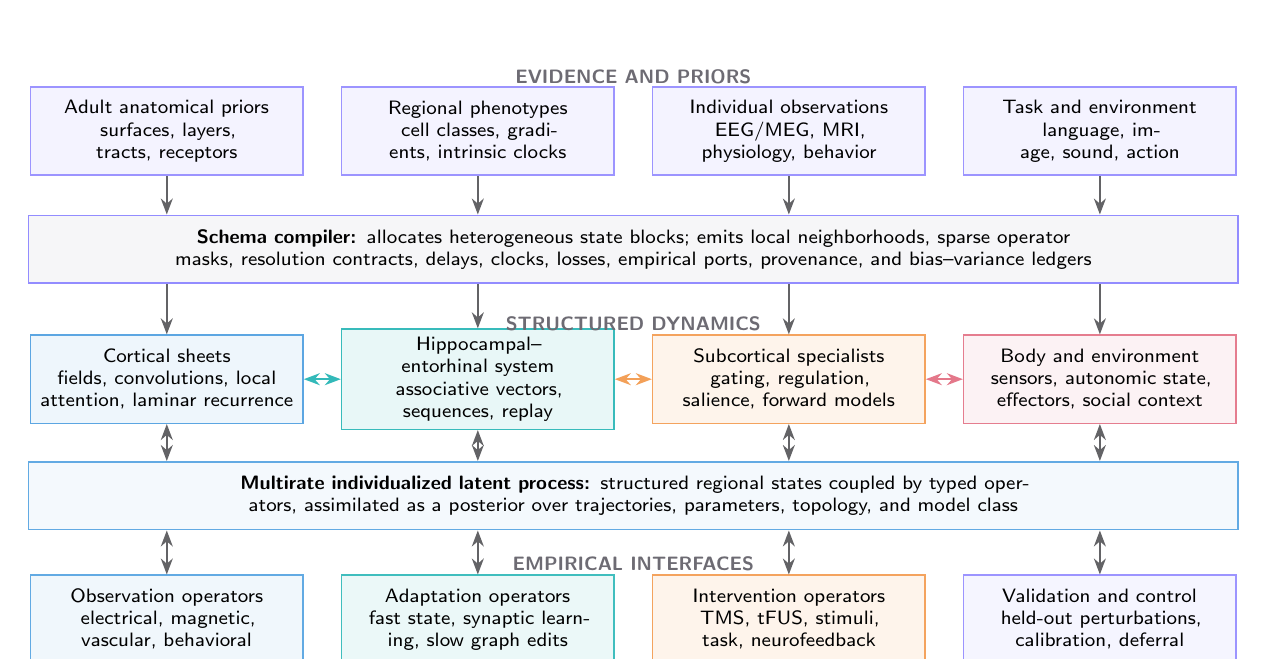
\begin{tikzpicture}[
  x=1cm,y=1cm,
  line cap=butt,line join=miter,
  font=\sffamily\scriptsize,
  box/.style={draw=ink!62,line width=.55pt,align=center,
              text width=3.25cm,minimum height=1.12cm,inner sep=3pt,fill=white},
  wide/.style={draw=ink!62,line width=.65pt,align=center,
               text width=15.15cm,minimum height=.86cm,inner sep=3pt},
  arrow/.style={->,>=Stealth,line width=.62pt,draw=ink!72},
  biarrow/.style={<->,>=Stealth,line width=.62pt,draw=ink!72}
]
% Evidence layer
\node[box,fill=frontpurple!8,draw=frontpurple!72] (adult) at (1.9,6.25)
  {Adult anatomical priors\\surfaces, layers, tracts, receptors};
\node[box,fill=frontpurple!8,draw=frontpurple!72] (phenotype) at (5.85,6.25)
  {Regional phenotypes\\cell classes, gradients, intrinsic clocks};
\node[box,fill=frontpurple!8,draw=frontpurple!72] (subject) at (9.80,6.25)
  {Individual observations\\EEG/MEG, MRI, physiology, behavior};
\node[box,fill=frontpurple!8,draw=frontpurple!72] (context) at (13.75,6.25)
  {Task and environment\\language, image, sound, action};

% Compiler
\node[wide,fill=papergray,draw=frontpurple!78] (compiler) at (7.825,4.75)
  {\textbf{Schema compiler:} allocates heterogeneous state blocks; emits local neighborhoods, sparse operator masks, resolution contracts, delays, clocks, losses, empirical ports, provenance, and bias--variance ledgers};

% Runtime modules
\node[box,fill=frontblue!8,draw=frontblue!75] (cortex) at (1.9,3.10)
  {Cortical sheets\\fields, convolutions, local attention, laminar recurrence};
\node[box,fill=frontteal!9,draw=frontteal!78] (hippo) at (5.85,3.10)
  {Hippocampal--entorhinal system\\associative vectors, sequences, replay};
\node[box,fill=frontorange!10,draw=frontorange!82] (subcortex) at (9.80,3.10)
  {Subcortical specialists\\gating, regulation, salience, forward models};
\node[box,fill=frontred!7,draw=frontred!72] (body) at (13.75,3.10)
  {Body and environment\\sensors, autonomic state, effectors, social context};

% State bus
\node[wide,fill=frontblue!5,draw=frontblue!72] (posterior) at (7.825,1.62)
  {\textbf{Multirate individualized latent process:} structured regional states coupled by typed operators, assimilated as a posterior over trajectories, parameters, topology, and model class};

% Empirical interfaces
\node[box,fill=frontblue!7,draw=frontblue!72] (observe) at (1.9,.05)
  {Observation operators\\electrical, magnetic, vascular, behavioral};
\node[box,fill=frontteal!8,draw=frontteal!75] (plasticity) at (5.85,.05)
  {Adaptation operators\\fast state, synaptic learning, slow graph edits};
\node[box,fill=frontorange!10,draw=frontorange!82] (intervene) at (9.80,.05)
  {Intervention operators\\TMS, tFUS, stimuli, task, neurofeedback};
\node[box,fill=frontpurple!7,draw=frontpurple!72] (eval) at (13.75,.05)
  {Validation and control\\held-out perturbations, calibration, deferral};

\foreach \n in {adult,phenotype,subject,context}{\draw[arrow] (\n.south)--(\n.south |- compiler.north);}
\foreach \n in {cortex,hippo,subcortex,body}{\draw[arrow] (compiler.south -| \n.north)--(\n.north);}
\foreach \n in {cortex,hippo,subcortex,body}{\draw[biarrow] (\n.south)--(\n.south |- posterior.north);}
\foreach \n in {observe,plasticity,intervene,eval}{\draw[biarrow] (posterior.south -| \n.north)--(\n.north);}
\draw[biarrow,frontteal!80] (cortex.east)--(hippo.west);
\draw[biarrow,frontorange!85] (hippo.east)--(subcortex.west);
\draw[biarrow,frontred!75] (subcortex.east)--(body.west);

\node[font=\sffamily\bfseries\scriptsize,text=muted] at (7.825,6.94) {EVIDENCE AND PRIORS};
\node[font=\sffamily\bfseries\scriptsize,text=muted] at (7.825,3.80) {STRUCTURED DYNAMICS};
\node[font=\sffamily\bfseries\scriptsize,text=muted] at (7.825,.75) {EMPIRICAL INTERFACES};
\end{tikzpicture}}
\caption{\textbf{Compiled whole-brain modeling framework.} Anatomical and phenotypic evidence defines a probabilistic adult-brain schema; individual observations and task context constrain its subject-specific state. A compiler maps the schema into heterogeneous memory regions, local cortical neighborhoods, sparse long-range operators, update clocks, and empirical interfaces. Runtime modules need not share a representation or resolution. Their contract is an explicit state type, operator family, spatial and temporal support, uncertainty semantics, and a validated boundary map.}
\label{fig:architecture}
\end{figure*}%
}

\newcommand{\StructuredStateFigure}{%
\begin{figure*}[t]
\centering
\resizebox{\textwidth}{!}{%
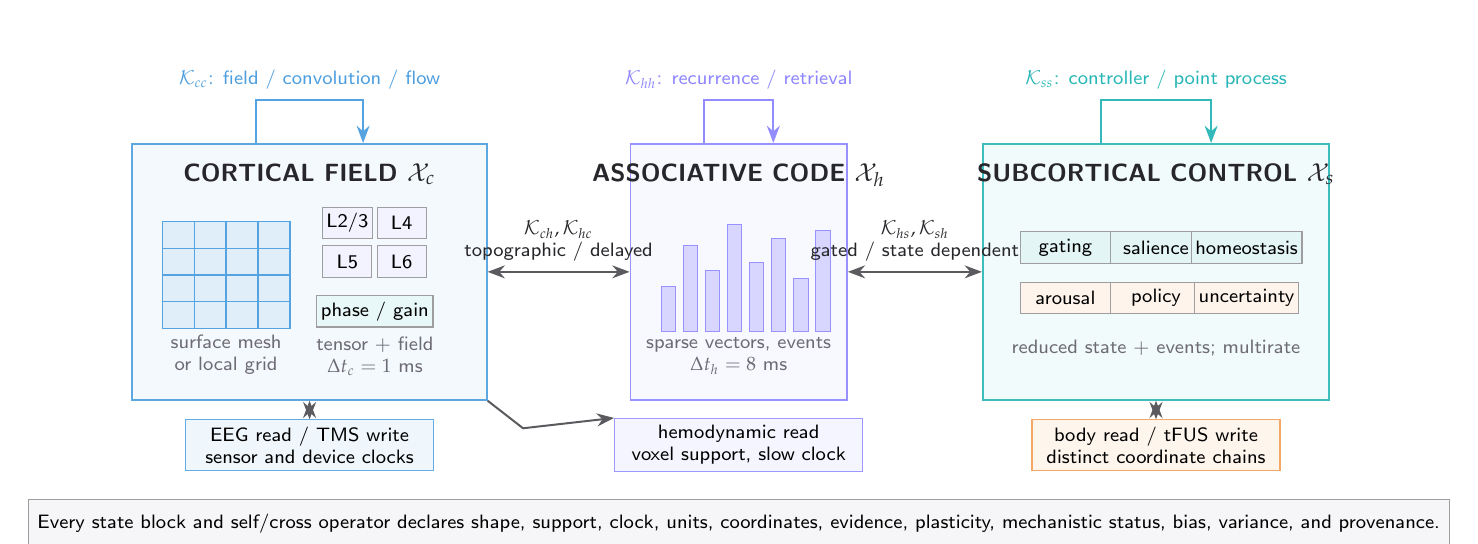
\begin{tikzpicture}[
  x=1cm,y=1cm,
  line cap=butt,line join=miter,
  font=\sffamily\scriptsize,
  region/.style={draw=ink!62,line width=.65pt,align=center,fill=white},
  cell/.style={draw=ink!45,minimum width=.62cm,minimum height=.40cm,
               inner sep=1.5pt,fill=white},
  port/.style={draw=ink!55,minimum height=.64cm,align=center,inner sep=2.5pt},
  arrow/.style={->,>=Stealth,line width=.72pt,draw=ink!76},
  biarrow/.style={<->,>=Stealth,line width=.72pt,draw=ink!76}
]
\node[region,minimum width=4.5cm,minimum height=3.25cm,
      fill=frontblue!5,draw=frontblue!74] (cortex) at (2.45,2.55) {};
\node[anchor=north,font=\sffamily\bfseries\small,text=ink] at (2.45,4.05)
  {CORTICAL FIELD \(\mathcal X_c\)};
\begin{scope}[shift={(.58,1.83)}]
  \fill[frontblue!14] (0,0) rectangle (1.62,1.36);
  \draw[frontblue!78,line width=.48pt] (0,0) grid[xstep=.405,ystep=.34] (1.62,1.36);
\end{scope}
\node[align=center,text=muted] at (1.39,1.50) {surface mesh\\or local grid};
\node[cell,fill=frontpurple!9] at (2.93,3.17) {L2/3};
\node[cell,fill=frontpurple!9] at (3.62,3.17) {L4};
\node[cell,fill=frontpurple!9] at (2.93,2.68) {L5};
\node[cell,fill=frontpurple!9] at (3.62,2.68) {L6};
\node[cell,minimum width=1.33cm,fill=frontteal!9] at (3.28,2.05) {phase / gain};
\node[align=center,text=muted] at (3.28,1.48) {tensor + field\\\(\Delta t_c=1\) ms};

\node[region,minimum width=2.75cm,minimum height=3.25cm,
      fill=frontpurple!5,draw=frontpurple!74] (hippo) at (7.90,2.55) {};
\node[anchor=north,font=\sffamily\bfseries\small,text=ink] at (7.90,4.05)
  {ASSOCIATIVE CODE \(\mathcal X_h\)};
\foreach \x/\h in {6.92/.58,7.20/1.10,7.48/.78,7.76/1.36,8.04/.88,8.32/1.18,8.60/.68,8.88/1.28}{
  \fill[frontpurple!28] (\x,1.79) rectangle ++(.18,\h);
  \draw[frontpurple!74,line width=.35pt] (\x,1.79) rectangle ++(.18,\h);
}
\node[align=center,text=muted] at (7.90,1.48) {sparse vectors, events\\\(\Delta t_h=8\) ms};

\node[region,minimum width=4.4cm,minimum height=3.25cm,
      fill=frontteal!5,draw=frontteal!76] (control) at (13.20,2.55) {};
\node[anchor=north,font=\sffamily\bfseries\small,text=ink] at (13.20,4.05)
  {SUBCORTICAL CONTROL \(\mathcal X_s\)};
\node[cell,minimum width=1.15cm,fill=frontteal!11] at (12.05,2.86) {gating};
\node[cell,minimum width=1.15cm,fill=frontteal!11] at (13.20,2.86) {salience};
\node[cell,minimum width=1.15cm,fill=frontteal!11] at (14.35,2.86) {homeostasis};
\node[cell,minimum width=1.15cm,fill=frontorange!10] at (12.05,2.22) {arousal};
\node[cell,minimum width=1.15cm,fill=frontorange!10] at (13.20,2.22) {policy};
\node[cell,minimum width=1.15cm,fill=frontorange!10] at (14.35,2.22) {uncertainty};
\node[align=center,text=muted] at (13.20,1.58) {reduced state + events; multirate};

\draw[biarrow] (cortex.east)--node[above,text=ink,align=center]
  {\(\mathcal K_{ch},\mathcal K_{hc}\)\\topographic / delayed} (hippo.west);
\draw[biarrow] (hippo.east)--node[above,text=ink,align=center]
  {\(\mathcal K_{hs},\mathcal K_{sh}\)\\gated / state dependent} (control.west);

\draw[arrow,frontblue!78] ([xshift=-.68cm]cortex.north)
  -- ([xshift=-.68cm,yshift=.55cm]cortex.north)
  -- node[above,text=frontblue!82]
  {\(\mathcal K_{cc}\): field / convolution / flow}
  ([xshift=.68cm,yshift=.55cm]cortex.north)
  -- ([xshift=.68cm]cortex.north);
\draw[arrow,frontpurple!78] ([xshift=-.44cm]hippo.north)
  -- ([xshift=-.44cm,yshift=.55cm]hippo.north)
  -- node[above,text=frontpurple!82]
  {\(\mathcal K_{hh}\): recurrence / retrieval}
  ([xshift=.44cm,yshift=.55cm]hippo.north)
  -- ([xshift=.44cm]hippo.north);
\draw[arrow,frontteal!80] ([xshift=-.70cm]control.north)
  -- ([xshift=-.70cm,yshift=.55cm]control.north)
  -- node[above,text=frontteal!84]
  {\(\mathcal K_{ss}\): controller / point process}
  ([xshift=.70cm,yshift=.55cm]control.north)
  -- ([xshift=.70cm]control.north);

\node[port,minimum width=3.15cm,fill=frontblue!7,draw=frontblue!70] (eeg) at (2.45,.35)
  {EEG read / TMS write\\sensor and device clocks};
\node[port,minimum width=3.15cm,fill=frontpurple!7,draw=frontpurple!70] (fmri) at (7.90,.35)
  {hemodynamic read\\voxel support, slow clock};
\node[port,minimum width=3.15cm,fill=frontorange!9,draw=frontorange!78] (tfus) at (13.20,.35)
  {body read / tFUS write\\distinct coordinate chains};
\draw[biarrow] (eeg.north)--(cortex.south);
\draw[arrow] (cortex.south east) -- ++(.45,-.35) -- (fmri.north west);
\draw[biarrow] (tfus.north)--(control.south);

\node[draw=ink!45,fill=papergray,align=center,
      minimum width=15.70cm,minimum height=.62cm] at (7.90,-.65)
  {Every state block and self/cross operator declares shape, support, clock, units, coordinates, evidence, plasticity, mechanistic status, bias, variance, and provenance.};
\end{tikzpicture}}
\caption{\textbf{Heterogeneous structured regions and operator-valued
connections.} Allocated regions need not have the same shape, dimensionality,
clock, or internal topology. Each self-connection and cross-region connection
selects its own transfer family and maps a documented boundary representation
into a compatible destination port. Observation and intervention ports attach
at their physical supports and clocks. The drawing shows three regions and
three empirical ports for clarity; the compiled graph may contain arbitrarily
sized and nested blocks at many resolutions.}
\label{fig:structuredstate}
\end{figure*}%
}

\newcommand{\ResolutionFigure}{%
\begin{figure*}[t]
\centering
\resizebox{\textwidth}{!}{%
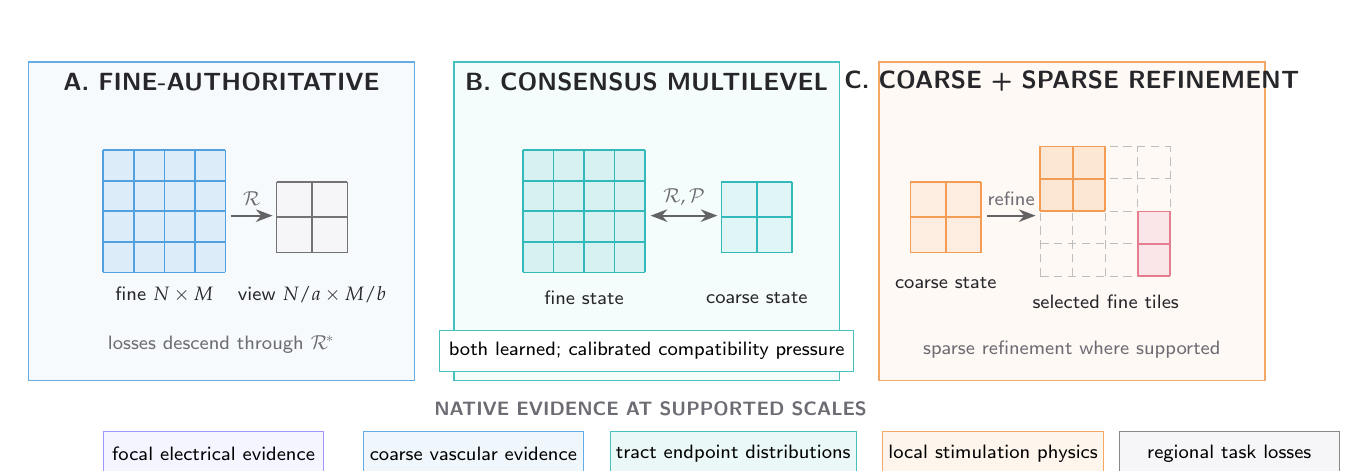
\begin{tikzpicture}[
  x=1cm,y=1cm,
  line cap=butt,line join=miter,
  font=\sffamily\scriptsize,
  panel/.style={draw=ink!58,line width=.6pt,minimum width=4.9cm,
                minimum height=4.05cm,fill=white},
  source/.style={draw=ink!50,align=center,minimum width=2.8cm,
                 minimum height=.55cm,inner sep=2pt},
  arrow/.style={->,>=Stealth,line width=.68pt,draw=ink!72},
  biarrow/.style={<->,>=Stealth,line width=.68pt,draw=ink!72}
]
\node[panel,fill=frontblue!4,draw=frontblue!70] (pa) at (2.55,2.65) {};
\node[panel,fill=frontteal!4,draw=frontteal!72] (pb) at (7.95,2.65) {};
\node[panel,fill=frontorange!5,draw=frontorange!78] (pc) at (13.35,2.65) {};

\node[font=\sffamily\bfseries\small,text=ink] at (2.55,4.42) {A. FINE-AUTHORITATIVE};
\node[font=\sffamily\bfseries\small,text=ink] at (7.95,4.42) {B. CONSENSUS MULTILEVEL};
\node[font=\sffamily\bfseries\small,text=ink] at (13.35,4.42) {C. COARSE + SPARSE REFINEMENT};

% Panel A grids
\begin{scope}[shift={(1.05,2.00)}]
  \fill[frontblue!16] (0,0) rectangle (1.55,1.55);
  \draw[frontblue!80,line width=.6pt] (0,0) grid[xstep=.3875,ystep=.3875] (1.55,1.55);
\end{scope}
\node[align=center,text=ink] at (1.825,1.72) {fine $N\times M$};
\begin{scope}[shift={(3.25,2.25)}]
  \fill[papergray] (0,0) rectangle (.90,.90);
  \draw[ink!65,line width=.6pt] (0,0) grid[xstep=.45,ystep=.45] (.90,.90);
\end{scope}
\node[align=center,text=ink] at (3.70,1.72) {view $N/a\times M/b$};
\draw[arrow] (2.67,2.72)--node[above,text=muted] {$\mathcal R$} (3.20,2.72);
\node[align=center,text=muted] at (2.55,1.08) {losses descend through $\mathcal R^{\!*}$};

% Panel B grids
\begin{scope}[shift={(6.38,2.00)}]
  \fill[frontteal!16] (0,0) rectangle (1.55,1.55);
  \draw[frontteal!80,line width=.6pt] (0,0) grid[xstep=.3875,ystep=.3875] (1.55,1.55);
\end{scope}
\node[align=center,text=ink] at (7.155,1.68) {fine state};
\begin{scope}[shift={(8.90,2.25)}]
  \fill[frontteal!12] (0,0) rectangle (.90,.90);
  \draw[frontteal!80,line width=.6pt] (0,0) grid[xstep=.45,ystep=.45] (.90,.90);
\end{scope}
\node[align=center,text=ink] at (9.35,1.68) {coarse state};
\draw[biarrow] (8.00,2.72)--node[above,text=muted] {$\mathcal R,\mathcal P$} (8.85,2.72);
\node[draw=frontteal!72,fill=white,align=center,minimum width=3.45cm,
      minimum height=.52cm] at (7.95,1.00) {both learned; calibrated compatibility pressure};

% Panel C grids
\begin{scope}[shift={(11.30,2.25)}]
  \fill[frontorange!16] (0,0) rectangle (.90,.90);
  \draw[frontorange!88,line width=.6pt] (0,0) grid[xstep=.45,ystep=.45] (.90,.90);
\end{scope}
\node[align=center,text=ink] at (11.75,1.86) {coarse state};
\draw[arrow] (12.27,2.72)--node[above,text=muted] {refine} (12.89,2.72);
\begin{scope}[shift={(12.95,1.95)}]
  \draw[ink!30,densely dashed] (0,0) grid[xstep=.4125,ystep=.4125] (1.65,1.65);
  \fill[frontorange!22] (0,.825) rectangle (.825,1.65);
  \draw[frontorange!88,line width=.6pt] (0,.825) grid[xstep=.4125,ystep=.4125] (.825,1.65);
  \fill[frontred!14] (1.2375,0) rectangle (1.65,.825);
  \draw[frontred!72,line width=.6pt] (1.2375,0) grid[xstep=.4125,ystep=.4125] (1.65,.825);
\end{scope}
\node[align=center,text=ink] at (13.78,1.62) {selected fine tiles};
\node[align=center,text=muted] at (13.35,1.02) {sparse refinement where supported};

% Heterogeneous evidence bar
\node[font=\sffamily\bfseries\scriptsize,text=muted] at (8.00,.27)
  {NATIVE EVIDENCE AT SUPPORTED SCALES};
\node[source,fill=frontpurple!7,draw=frontpurple!70] (eeg) at (2.45,-.30)
  {focal electrical evidence};
\node[source,fill=frontblue!7,draw=frontblue!70] (fmri) at (5.75,-.30)
  {coarse vascular evidence};
\node[source,fill=frontteal!8,draw=frontteal!72] (tract) at (9.05,-.30)
  {tract endpoint distributions};
\node[source,fill=frontorange!9,draw=frontorange!78] (stim) at (12.35,-.30)
  {local stimulation physics};
\node[source,fill=papergray,draw=ink!55] (task) at (15.35,-.30)
  {regional task losses};
\end{tikzpicture}}
\caption{\textbf{Three multiresolution state semantics.} “Resolution” is not
limited to preprocessing. A fine-authoritative field materializes derived
coarse views; a consensus model gives multiple levels their own degrees of
freedom under continuous agreement pressure; a coarse-authoritative model
instantiates only selected high-resolution tiles. The schema declares the
authority policy, projection operators, gradient routes, uncertainty, and
refinement triggers. Every view and map carries separate bias and variance
terms. Heterogeneous observations attach at the levels their
physical point-spread functions justify. Two dyadic grids are drawn for
clarity; actual views may use any number of non-dyadic, non-grid, and
source-specific scales, and need not admit one consistent global field.}
\label{fig:resolution}
\end{figure*}%
}

\newcommand{\TimescaleFigure}{%
\begin{figure}[t]
\centering
\resizebox{\columnwidth}{!}{%
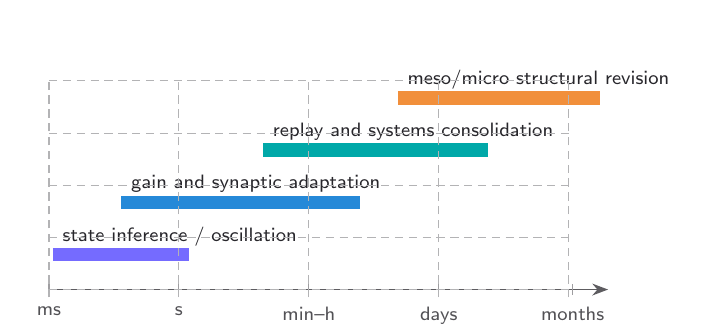
\begin{tikzpicture}[font=\sffamily\scriptsize,x=1cm,y=.72cm,line cap=butt,line join=miter]
  \draw[->,>=Stealth,line width=.6pt,draw=ink!75] (0,0)--(7.1,0);
  \foreach \x/\lab in {0/ms,1.65/s,3.3/min--h,4.95/days,6.65/months}{
    \draw[ink!45] (\x,.09)--(\x,-.09) node[below=1pt,text=ink!80]{\lab};
  }
  \draw[line width=4.8pt,frontpurple] (.05,.62)--(1.78,.62);
  \node[anchor=west,text=ink] at (.05,.94) {state inference / oscillation};
  \draw[line width=4.8pt,frontblue] (.92,1.54)--(3.95,1.54);
  \node[anchor=west,text=ink] at (.92,1.86) {gain and synaptic adaptation};
  \draw[line width=4.8pt,frontteal] (2.72,2.46)--(5.58,2.46);
  \node[anchor=west,text=ink] at (2.72,2.78) {replay and systems consolidation};
  \draw[line width=4.8pt,frontorange] (4.43,3.38)--(7.0,3.38);
  \node[anchor=west,text=ink] at (4.43,3.70) {meso/micro structural revision};
  \draw[densely dashed,ink!35] (0,-.14) grid[xstep=1.65,ystep=.92] (6.6,3.75);
\end{tikzpicture}}
\caption{\textbf{Nested adaptive timescales.} The architecture distinguishes fast latent dynamics, intermediate gain and synaptic changes, consolidation, and conservative structural revision. Ranges overlap and depend on subsystem and task; the bars are scheduler classes rather than universal biological constants.}
\label{fig:timescales}
\end{figure}%
}

\newcommand{\FrameGraphFigure}{%
\begin{figure*}[t]
\centering
\resizebox{.98\textwidth}{!}{%
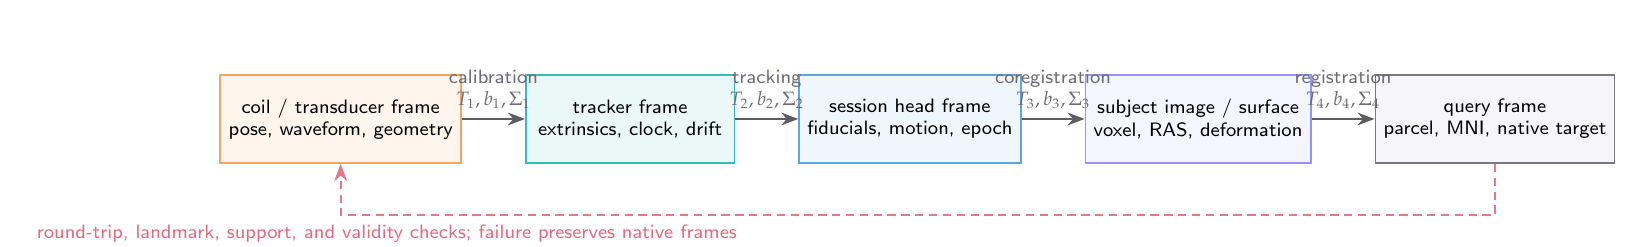
\begin{tikzpicture}[
  font=\sffamily\scriptsize,
  line cap=butt,line join=miter,
  node distance=8mm,
  frame/.style={draw=ink!62,line width=.6pt,minimum width=2.65cm,
                minimum height=1.12cm,align=center,inner sep=3pt,fill=white},
  edge/.style={->,>=Stealth,line width=.7pt,draw=ink!75}
]
\node[frame,fill=frontorange!9,draw=frontorange!80] (device)
  {coil / transducer frame\\pose, waveform, geometry};
\node[frame,fill=frontteal!8,draw=frontteal!78,right=of device] (tracker)
  {tracker frame\\extrinsics, clock, drift};
\node[frame,fill=frontblue!7,draw=frontblue!75,right=of tracker] (head)
  {session head frame\\fiducials, motion, epoch};
\node[frame,fill=frontpurple!7,draw=frontpurple!74,right=of head] (image)
  {subject image / surface\\voxel, RAS, deformation};
\node[frame,fill=papergray,draw=ink!62,right=of image] (atlas)
  {query frame\\parcel, MNI, native target};
\draw[edge] (device)--node[above,align=center,text=muted]
  {calibration\\\(T_1,b_1,\Sigma_1\)} (tracker);
\draw[edge] (tracker)--node[above,align=center,text=muted]
  {tracking\\\(T_2,b_2,\Sigma_2\)} (head);
\draw[edge] (head)--node[above,align=center,text=muted]
  {coregistration\\\(T_3,b_3,\Sigma_3\)} (image);
\draw[edge] (image)--node[above,align=center,text=muted]
  {registration\\\(T_4,b_4,\Sigma_4\)} (atlas);
\draw[frontred!75,line width=.72pt,densely dashed,->,>=Stealth]
  (atlas.south) -- ++(0,-.65) -| node[below,pos=.48,text=frontred!82]
  {round-trip, landmark, support, and validity checks; failure preserves native frames}
  (device.south);
\end{tikzpicture}}
\caption{\textbf{Coordinate and calibration frame graph.} Device commands,
tracked pose, head coordinates, subject images, and atlas or query coordinates
remain distinct nodes connected by versioned transforms. Each edge retains
calibration observations, epoch, systematic offset, random covariance, and
model discrepancy. Composition is query-specific; raw transforms are never
multiplied away, and a failed cycle prevents a global coordinate claim.}
\label{fig:framegraph}
\end{figure*}%
}

\newcommand{\ClosedLoopFigure}{%
\begin{figure*}[t]
\centering
\resizebox{.97\textwidth}{!}{%
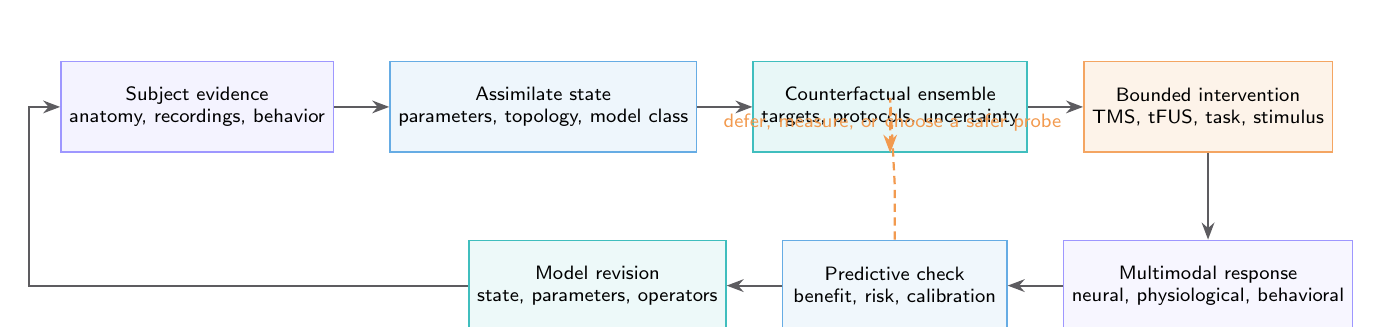
\begin{tikzpicture}[
  font=\sffamily\scriptsize,
  line cap=butt,line join=miter,
  node distance=6mm and 7mm,
  stage/.style={draw=ink!60,line width=.55pt,minimum width=2.85cm,
                minimum height=1.15cm,align=center,inner sep=3pt,fill=white},
  arrow/.style={->,>=Stealth,line width=.7pt,draw=ink!75}
]
\node[stage,fill=frontpurple!8,draw=frontpurple!70] (data) {Subject evidence\\anatomy, recordings, behavior};
\node[stage,fill=frontblue!8,draw=frontblue!70,right=of data] (infer) {Assimilate state\\parameters, topology, model class};
\node[stage,fill=frontteal!9,draw=frontteal!75,right=of infer] (simulate) {Counterfactual ensemble\\targets, protocols, uncertainty};
\node[stage,fill=frontorange!11,draw=frontorange!80,right=of simulate] (act) {Bounded intervention\\TMS, tFUS, task, stimulus};
\node[stage,fill=frontpurple!6,draw=frontpurple!70,below=11mm of act] (response) {Multimodal response\\neural, physiological, behavioral};
\node[stage,fill=frontblue!7,draw=frontblue!70,left=of response] (check) {Predictive check\\benefit, risk, calibration};
\node[stage,fill=frontteal!7,draw=frontteal!75,left=of check] (update) {Model revision\\state, parameters, operators};
\draw[arrow] (data)--(infer);
\draw[arrow] (infer)--(simulate);
\draw[arrow] (simulate)--(act);
\draw[arrow] (act)--(response);
\draw[arrow] (response)--(check);
\draw[arrow] (check)--(update);
\draw[arrow] (update.west)-|([xshift=-4mm]data.west)|-(data.west);
\draw[frontorange!90,line width=.8pt,densely dashed,->,>=Stealth]
  (check.north) -- ++(0,7mm)
  -- node[above,text=frontorange!90]{defer, measure, or choose a safer probe}
  ([yshift=7mm]simulate.south) -- (simulate.south);
\end{tikzpicture}}
\caption{\textbf{Closed-loop individualization.} Measurements constrain a posterior over latent state, parameters, topology, and model class. Candidate actions are evaluated across posterior models, applied only through bounded protocols, measured multimodally, and used to revise the model. Clinical or wellness claims require prospective decision-level validation beyond successful signal reconstruction.}
\label{fig:closedloop}
\end{figure*}%
}


\begin{document}
\thispagestyle{versionsix}

\noindent\colorbox{ink}{\parbox{\dimexpr\textwidth-2\fboxsep\relax}{%
  \color{white}\sffamily\bfseries\fontsize{10.5}{12}\selectfont
  SuperCognition Labs\hfill SC-WBD \textperiodcentered\ VERSION 6}}

\vspace{7mm}
{\sffamily\bfseries\fontsize{9}{10}\selectfont\color{frontpurple}
TECHNICAL THESIS AND DEVELOPMENT PROGRAM\par}
\vspace{3mm}
{\leftskip=1em\noindent\sffamily\bfseries\fontsize{23}{26}\selectfont\color{ink}
Integrated Whole-Brain Modeling Across\\
Modalities, Scales, and Dynamics for\\
Individualized Neurotechnology\par}
\vspace{3mm}
{\sffamily\fontsize{13}{15}\selectfont\color{muted}
A falsifiable scientific position, executable data contract, and implementation roadmap\par}

\vspace{6mm}
{\sffamily\bfseries\fontsize{12}{14}\selectfont\color{ink}Jacob Valdez\par}
{\sffamily\fontsize{9}{11}\selectfont\color{muted}
Founding Architect, SuperCognition Labs\quad\textperiodcentered\quad
\href{mailto:jacob@supercognitionlabs.com}{jacob@supercognitionlabs.com}\par}

\vspace{4mm}
\noindent\begin{tabularx}{\textwidth}{@{}>{\sffamily\bfseries\color{muted}}p{.15\textwidth}X>{\sffamily\bfseries\color{muted}}p{.11\textwidth}p{.26\textwidth}@{}}
STATUS & \draftbadge & DOCUMENT & Thesis / position /\newline implementation contract\\
CLAIM STATE & No empirical result is asserted & RELEASE & V6\\
\end{tabularx}

\vspace{4mm}\hrule\vspace{4mm}
{\sffamily\bfseries\fontsize{9}{10}\selectfont\color{frontpurple}ABSTRACT\par}
\vspace{2mm}
{\fontsize{9.1}{11.25}\selectfont\color{ink}
Magnetic resonance imaging, electroencephalography, transcranial magnetic stimulation, and transcranial focused ultrasound neither observe nor perturb the human brain at commensurate spatial or temporal resolutions. Structural MRI constrains anatomy; fMRI samples blurred vascular consequences over seconds; EEG resolves electrical dynamics over milliseconds through an ill-posed forward model; TMS delivers a state-dependent electric field; and tFUS delivers acoustically distorted exposure with device- and skull-dependent uncertainty. This thesis proposes \textbf{SuperCognition Whole-Brain Dynamics (SC-WBD)} as a human-adult model family for relating these methods without pretending that they occupy one raster, clock, coordinate frame, or biological level.

SC-WBD treats a region as a structured, scale-indexed state space rather than a scalar node. Cortical fields, laminar tensors, event processes, associative codes, vascular compartments, and reduced control states communicate through typed operators compiled from a probabilistic anatomical schema. Evidence remains authoritative at its native scale. Fine-authoritative, multilevel-consensus, and coarse-with-sparse-refinement policies allow several resolutions to coexist; calibrated transforms move predictions, gradients, and uncertainty across supports without manufacturing fine truth from coarse measurements. Each source, transform, observation, intervention, and learned residual carries provenance, variance, bias bounds, and model-discrepancy assumptions.

The central claim is deliberately falsifiable: joint, multirate inference should identify selected coupling and delay parameters more reliably than isolated modalities or naive resampling, and a calibrated perturbation should recover distinctions that passive measurements leave unresolved. The first required evidence is therefore a three-region linear--Gaussian recovery benchmark with EEG-like fast mixing, fMRI-like delayed hemodynamics, and an impulse intervention, followed by an end-to-end synthetic compiler demonstration. Both have now been run, and they narrow the central claim: what they support is source-native \emph{clock} handling over resampling, whereas in that deliberately small system the second modality supplies roughly one percent of the electrical channel's information about coupling---consumed by its own observation nuisances---and effectively none about the conduction delay, and the impulse's apparent advantage is accounted for by its input energy. These are results about a synthetic design, and about a design shaped to one of its two modalities; no empirical result about brains is asserted. The architecture rejects undeclared units or frames, unsupported prolongation, intervention-free causal labels, unconstrained mechanistic residuals, invalid leakage splits, and cross-scale gluing that fails declared commutation tolerances.

This document states the implementation contracts, rejection conditions, experimental gates, and staged training program. Heterogeneous public, partnered, prospective, and simulated trajectories may supervise only the modules and ports they observe; missing states are marginalized rather than labeled. The near-term objective is calibrated cross-method prediction and bounded TMS/tFUS target comparison, not an unrestricted digital brain. Longer-term language, affective, social, and person-specific models remain downstream hypotheses whose credibility depends on prospective neural, physiological, behavioral, and intervention forecasts.\par}

\vspace{4mm}
{\sffamily\bfseries\fontsize{7.4}{8.5}\selectfont\color{muted}KEYWORDS}\par
{\sffamily\fontsize{8.2}{10}\selectfont\color{muted}
whole-brain modeling; heterogeneous data fusion; multiscale neural dynamics; identifiability; uncertainty quantification; individualized neurotechnology; neuromodulation; computational neuroscience\par}

\clearpage
\twocolumn
\small

\section{0. Program Thesis, Claim Boundary, and Implementation Contract}

This document is not a report that SC-WBD has already achieved whole-brain
prediction. It is the technical thesis that governs what SuperCognition Labs
will build, what evidence may update it, which configurations the compiler
must reject, and which experiments are capable of changing the program's
scientific commitments. Its first audience is therefore dual: researchers
should be able to locate the assumptions that require evidence, while
implementation agents should be able to translate each contract into schemas,
validators, tests, and acceptance gates.

The thesis has four load-bearing commitments. First, heterogeneous methods are
related through a latent generative process and method-specific read/write
operators, not through naive resampling into a common tensor. Second, adult
human anatomy supplies strong probabilistic topology and phenotype priors,
while effective coupling, local computation, state, and slow plasticity remain
learnable. Third, resolution is an indexed property of state and evidence:
several non-equivalent spatial and temporal supports may coexist without a
single materialized truth. Fourth, mechanistic language is earned only by
predictions that an equal-capacity surrogate misses, especially under held-out
perturbation. These commitments are compatible with useful predictive models
that remain agnostic about many biological details; they do not license a
claim that every admitted operator is neurally realized.

\begin{table*}[t]
\centering
\footnotesize
\setlength{\tabcolsep}{4pt}
\renewcommand{\arraystretch}{1.10}
\begin{tabularx}{\textwidth}{@{}p{.19\textwidth}p{.27\textwidth}p{.27\textwidth}X@{}}
\toprule
\textbf{Program claim} & \textbf{Evidence that can support it} &
\textbf{Result that weakens or falsifies it} & \textbf{Implementation consequence}\\
\midrule
Typed, source-native fusion is preferable to naive resampling &
Better held-out likelihood, calibration, delay recovery, and intervention
forecast at matched compute and parameter count, measured against a tuned
resampling baseline. Adding a modality is not itself evidence: under (T4) it
cannot reduce information &
No reproducible gain over single-modality or carefully tuned resampling
baselines; increased overconfidence or negative transfer &
Retain only the provenance/type system; narrow or remove the shared latent
fusion claim. \emph{Narrowed on measured evidence to a claim about
source-native clocks; see Section 11.5}\\

Anatomical topology improves inference &
Data efficiency, out-of-distribution calibration, and causal forecast beyond
dense, randomized, and distance-matched graphs &
Equal-capacity controls match or exceed performance, or topology errors are
absorbed by residuals &
Demote anatomy from compiled constraint to weak prior for the affected scale\\

Multiresolution state adds information rather than decoration &
Native-scale prediction, calibrated refinement, boundary agreement, and
compute savings without hidden high-frequency hallucination &
Fine views cannot improve supported observables, fail round-trip tests, or
become overconfident outside measured tiles &
Disable the scale relation or use source-specific views without gluing\\

Perturbation reduces non-identifiability &
Rank/eigenvalue improvement in Fisher information \emph{at matched input
energy}, and prospective recovery of direction, delay, gain, dose, and state
dependence &
Intervention fails to distinguish posterior models, adds only field-model
uncertainty, or loses its apparent advantage against an energy-matched control &
Narrow the identifiable parameter set and redesign the perturbation rather
than reporting a causal estimate\\

Individualization improves future prediction &
Incremental calibrated log score and decision utility on new sessions and
unseen tasks or interventions &
Anatomy-only, population, or session-adapted baselines perform equivalently &
Do not label the model an individual twin; retain only the supported level of
adaptation\\
\bottomrule
\end{tabularx}
\caption{\textbf{Claims with consequences.} Each central commitment has a
measurement capable of making it smaller. Engineering breadth, parameter
count, plausible diagrams, and in-sample fit are not substitutes for these
tests. Rows 1 and 4 have been narrowed since the previous version because the
measurement was run and returned a smaller result than the claim; the evidence
columns record the controls that narrowing showed to be mandatory
(Section 11.5).}
\label{tab:claim-gates}
\end{table*}

\subsection{0.1 What SC-WBD Forbids}

A type system earns credibility by rejecting programs. SC-WBD therefore
distinguishes an operator family that can be represented from a model instance
that is admissible for a particular scientific claim. The compiler must fail
closed on the following conditions unless the schema explicitly changes the
claim class and records the override.

\begin{table*}[t]
\centering
\footnotesize
\setlength{\tabcolsep}{4pt}
\renewcommand{\arraystretch}{1.09}
\begin{tabularx}{\textwidth}{@{}p{.22\textwidth}p{.31\textwidth}X@{}}
\toprule
\textbf{Rejected configuration} & \textbf{Why it is scientifically invalid} &
\textbf{Required remedy}\\
\midrule
Unknown units, clock, physical support, frame, handedness, or transform lineage &
Numerical compatibility would be mistaken for measurement compatibility &
Supply a calibrated manifest with validity interval and uncertainty, or keep
the source disconnected from the requested path\\

Prolongation without a declared restriction partner and tested coverage &
A coarse observation would be converted into unsupported fine structure &
Provide paired maps, round-trip and held-out landmark tests, and an
out-of-support uncertainty policy; otherwise return a distribution or refuse\\

Global cross-scale state when overlap/cocycle residual exceeds tolerance &
Conflicting local views would be hidden by one raster &
Preserve separate sections, branch or marginalize the posterior, and emit an
obstruction certificate identifying the failed path\\

Effective or causal operator estimated from passive correlation alone &
Common input, observation mixing, and omitted state remain alternatives &
Label the object functional/statistical, or add an identified intervention or
assumption set sufficient for the causal claim\\

Learned residual allowed to dominate a mechanistic term silently &
The named mechanism becomes unfalsifiable &
Enforce a preregistered energy/gain ratio
\(\|\mathcal R_\theta\|/\|\mathcal F_{\rm mech}\|\leq\rho_{\max}\) on the
declared validity set, report violations, or reclassify the entire module as a
surrogate\\

Adaptive step sizes for a learned propagator without semigroup testing &
Coarse and composed fine transitions need not describe the same dynamics &
Measure the semigroup residual at every permitted step pair; restrict the
scheduler or include the discrepancy in prediction intervals\\

Population, subject, and session effects without centering or shrinkage &
The additive decomposition is not identified &
Use centered/sum-to-zero constraints or proper hierarchical priors and test
recovery in simulation\\

Bias assigned a point estimate without an estimator or external bound &
Calibration and model discrepancy can trade off non-identifiably &
Classify the term as design-estimable, externally bounded, or
prior-specified sensitivity; propagate the last category as a range\\

Pseudo-likelihood compatibility treated as a calibrated posterior likelihood &
Agreement penalties do not define a generative noise model &
Report a generalized/pseudo-posterior and calibrate it empirically, or validate
and promote the factor to a generative likelihood\\

Derived scans, sessions, relatives, stimuli, or simulator replicas crossing a
parent-level holdout &
Duplicated evidence produces invalid confidence and shortcut prediction &
Group by immutable lineage identifiers before splitting and fail the run when
parentage is unresolved\\

Intervention optimization outside an independently validated feasible set &
A learned objective cannot guarantee device, exposure, or protocol safety &
Require \(u\in\mathcal A_{\rm safe}\), independent safety checks, deferral,
and the applicable ethics and regulatory review\\
\bottomrule
\end{tabularx}
\caption{\textbf{Mandatory modeling refusals.} These are compiler and runtime
errors, not optional governance prose. An override changes the claim carried
by the resulting artifact and remains visible in its provenance.}
\label{tab:compiler-refusals}
\end{table*}

\subsection{0.2 Position Relative to Existing Model Families}

The latent-state/observation-operator decomposition is not new. Dynamic causal
modeling (DCM) already formalizes Bayesian inference over hidden neuronal
dynamics, effective connectivity, experimental inputs, and modality-specific
forward models \citep{friston2003dcm}. The Virtual Brain provides an
individualizable connectome-coupled simulation environment
\citep{sanz2013,sanz2015}; neurolib and BrainPy provide extensible machinery
for whole-brain neural-mass and general brain-dynamics programming
\citep{cakan2023neurolib,wang2023brainpy}. NeuroML/LEMS and PyNN establish
substantial prior art for declarative, unit-aware, simulator-independent model
specification \citep{cannon2014lems,davison2009pynn}. SC-WBD should interoperate
with these ecosystems rather than redescribe them as absent.

The proposed differentiator is the joint compilation of (i) heterogeneous
operator-valued regional state; (ii) non-nested, source-native spatial and
temporal resolutions; (iii) uncertain coordinate/clock/field transforms;
(iv) data-use provenance into gradient permissions and leakage barriers; and
(v) explicit claim-dependent refusal rules. DCM remains the clearest
statistical ancestor for generative inversion; declarative neuroscience
languages are the clearest software ancestor for typed execution. SC-WBD's
burden is to demonstrate that extending those ideas to multirate,
multiresolution, intervention-aware fusion yields identifiable and calibrated
predictions unavailable to simpler constructions.

Patient-specific cardiac modeling is a useful neighboring discipline because
it has had to separate code verification, physical validation, parameter
calibration, model-form uncertainty, and context-of-use credibility before a
digital-twin claim can influence a decision \citep{galappaththige2022}. SC-WBD
adopts the same ladder: numerical correctness is necessary; agreement with
recorded signals is stronger; held-out perturbation is stronger still; and
prospective decision improvement is a distinct claim.

\subsection{0.3 Identifiability Before Scale}

The first scientific artifact is intentionally small. Consider three latent
regional states with directed coupling, one unknown conduction delay, and a
controlled input:

\[
\begin{aligned}
\mathrm d x(t)={}&A(\vartheta)x(t)\,\mathrm dt
+B\,u(t-\tau_u)\,\mathrm dt\\
&+Q^{1/2}\mathrm dW_t,
\qquad x(t)\in\mathbb R^3 .
\end{aligned}
\tag{T1}
\]

An EEG-like instrument observes rapid instantaneous mixing,

\[
y_E[k]=L(\ell)x(k\Delta_E)+\epsilon_E[k],
\qquad \Delta_E=1~\mathrm{ms},
\tag{T2}
\]

whereas an fMRI-like instrument observes a slow hemodynamic convolution,

\[
y_B[n]=M\!\int_0^{T_h}h(s;\rho)x(n\Delta_B-s)\,\mathrm ds
+\epsilon_B[n],
\qquad \Delta_B=1~\mathrm{s}.
\tag{T3}
\]

The unknown vector \(\vartheta\) contains selected coupling gains and the
network delay, while \(\ell\) and \(\rho\) contain observation nuisance
parameters. For a linear--Gaussian discretization the expected Fisher
information for design \(d\) is

\[
\mathcal I_d(\eta)=
\sum_{m\in d}J_m(\eta)^\top R_m^{-1}J_m(\eta)
+\mathcal I_{\rm prior},
\quad
J_m=\frac{\partial\mu_m}{\partial\eta},
\tag{T4}
\]

with \(\eta=(\vartheta,\ell,\rho)\).

Two properties of (T4) must be stated where it is introduced, because a
benchmark that ignores either of them will report an artifact of its own
construction as a finding.

\textbf{Modality additivity is an identity, not a hypothesis.} Written as a sum
of per-modality quadratic forms, (T4) treats the modalities as conditionally
independent given \(\eta\). Each summand is positive semidefinite, so
\(\mathcal I_{\rm EEG+BOLD}
=\mathcal I_{\rm EEG}+\mathcal I_{\rm BOLD}-\mathcal I_{\rm prior}
\succeq\mathcal I_{\rm EEG}\)
holds algebraically, for every parameterization, every dataset, and every
truth. ``Joint is at least as informative as single-modality'' therefore cannot
fail, and a benchmark reporting it as a validated result reports a tautology.
The non-trivial part of joint information is the EEG/BOLD cross-covariance
induced by \emph{shared process noise}, which the block-diagonal form omits;
obtaining it requires whitening the stacked record rather than each modality
separately. The benchmark computes both and reports their difference, which is
exactly the amount by which (T4) over-counts. The discriminating comparisons
are consequently native versus resampled clocks, the \emph{size} of the second
modality's contribution to the preregistered subset, impulse versus no impulse
at matched input energy, and whether any added information becomes calibrated
recovery.

\textbf{A continuous conduction delay is a precondition for delay
identifiability.} The Fisher information of \(\tau\) exists only if
\(\partial\mu/\partial\tau\) exists. If \(\tau\) is quantized to the sample
grid, that derivative is identically zero and the delay carries \emph{no}
information under any design---including designs that would otherwise recover
it well. A benchmark built on a quantized delay would report zero delay
information for every design and mistake an implementation choice for a
scientific result. (T1) and (T4) therefore require a fractional-delay
implementation; here a normalized Gaussian-windowed-sinc interpolation over the
history taps, so that \(\tau\) is a continuous parameter with a smooth
derivative. The 1\,s resampled design is retained precisely because it violates
this condition, and is reported as the illustration of what the violation looks
like rather than as a measurement of the delay.

The benchmark compares EEG alone, fMRI alone, joint native-clock inference,
joint inference after naive resampling, joint inference plus one calibrated
impulse, and---required rather than optional---the same impulse at total input
energy matched to the impulse-free design by scaling the background drive.
Without that sixth design, an impulse comparison measures the energy budget and
not the perturbation. A charitable resampling control, which discards EEG onto
the 1\,s grid but retains the exact fine-grained forward model, separates
information lost by decimation from bias introduced by the wrong
discretization. The benchmark reports rank, condition number, minimum non-prior
eigenvalue, parameter-profile likelihoods, posterior correlations, interval
coverage, and delay error. Prior contribution is shown separately so a
full-rank posterior cannot disguise a prior-dominated likelihood.

\textbf{What this system cannot be asked.} The state is three regions with no
spatial structure, and \(\vartheta\) is a few coupling gains plus one
conduction delay. That is an electrophysiological question, and a hemodynamic
instrument is being scored on it. The strengths such an instrument actually
has---spatial extent and localization, slow state, and constraining the very
observation model on which electrical source inversion depends---have nowhere
to appear in a three-region linear--Gaussian system. A weak fusion result
obtained here is therefore a correct statement about \emph{this design}. It is
not a general finding that cross-method integration is unprofitable, and it may
not be reported as one; reaching that stronger question requires extending the
system, not rerunning this one.

This is a planned calculation, not a favorable result assumed in advance. The
central premise is supported only if native-clock fusion or intervention
increases likelihood information for a preregistered parameter subset and
improves calibrated recovery across held-out simulation regimes. If it does
not, the compiler may still be useful as a provenance system, but the claim
that cross-method integration resolves those dynamics must be narrowed. That
calculation has now been performed in the linear--Gaussian case; its outcome,
and the narrowing this paragraph prescribes, are reported in Section 11.5. The
paragraph is left exactly as written, because it is the commitment against
which the result is being judged.

The second artifact compiles the same system from a source schema and performs
end-to-end recovery. It introduces known transform bias, shared session
calibration error, missing windows, unequal supports, and a deliberately
misspecified residual. Success requires: no leakage across simulated parent
subjects; recovery intervals with nominal coverage; lower held-out log loss
than single-method and naive-resampling baselines; detection of the
misspecified module; and refusal of at least one invalid schema. This synthetic
case is the minimum integration test for all later human experiments. It has
been built and run: three of the five criteria listed here were met, interval
coverage was not, the held-out log-loss comparison could not be evaluated
because none of the fits it compares had converged, and a sixth
subgroup-calibration criterion added by the implementation was met
(Section 11.5).

\subsection{0.4 Executable Evidence, Transform, and Gradient Contracts}

Every dataset snapshot is compiled from a source card rather than passed to a
global dataloader. A source card declares identity and hashes, participant and
derivative lineage, governance, native signal and units, spatial support,
point-spread function, clock, coordinate/calibration graph, observation or
intervention model, missingness, validity domain, bias/variance/discrepancy
ledger, permitted module and scale targets, and a fixed role: prior,
likelihood, boundary target, distillation, calibration, negative control, or
evaluation only. The compiler converts those declarations into dataloaders,
transform paths, loss factors, gradient masks, and group-aware splits. An
unknown field remains unknown; it is not supplied as zero or as an average
brain label.

The uncertainty ledger uses three different statuses. A quantity is
\textbf{design-estimable} only when the acquisition contains the replication,
randomization, intervention, anchor, or hierarchy necessary to estimate it.
Repeated sessions, for example, can estimate within- and between-session
variance but do not by themselves identify absolute model bias. A term is
\textbf{externally bounded} when a phantom, calibration target, independent
instrument, or negative control supplies a defensible interval. A term is
\textbf{prior-specified sensitivity} when neither is available; it is swept
over a declared range and cannot be advertised as empirically estimated.
Model discrepancy and calibration parameters are generally confounded without
informative assumptions, a known failure mode in computer-model calibration
\citep{kennedy2001,brynjarsdottir2014}.

For a derived quantity \(z=f(x,c)\), calibration uncertainty may be shared
across every observation in a session. First-order propagation therefore
retains cross-covariance:

\[
\begin{aligned}
\Sigma_z\approx{}&J_x\Sigma_xJ_x^\top+J_c\Sigma_cJ_c^\top\\
&+J_x\Sigma_{xc}J_c^\top+J_c\Sigma_{cx}J_x^\top,\\
b_z\approx{}&J_xb_x+J_cb_c+\delta_f .
\end{aligned}
\tag{T5}
\]

The transform graph stores each edge separately. Paths are checked for units,
handedness, epoch, support, round-trip residual, and calibration validity;
their composed result never replaces the original edges. Figure
\ref{fig:framegraph} gives the frame path used by the running example.

\FrameGraphFigure

For episode \(e\), only authorized additive factors are active:

\[
\begin{aligned}
\mathcal L=\sum_e w_e\bigl[&
\lambda_{\rm like}\mathcal L_{\rm like}^{(e)}
+\lambda_{\rm boundary}\mathcal L_{\rm boundary}^{(e)}\\
&+\lambda_{\rm distill}\mathcal L_{\rm distill}^{(e)}
+\lambda_{\rm cal}\mathcal L_{\rm cal}^{(e)}\\
&+\lambda_{\rm mech}\mathcal R_{\rm mech}^{(e)}
+\lambda_{\rm scale}\mathcal R_{\rm scale}^{(e)}\bigr].
\end{aligned}
\tag{T6}
\]

Weights depend on effective independent evidence and declared reliability, not
row count. Gradient conflict is logged by source and module. A conflict may
produce partial pooling, a source-specific adapter, a frozen path, a branched
posterior, or rejection; consensus is not mandatory.

\subsection{0.5 Running Case: Individual DLPFC TMS Targeting}

The running case asks a bounded question: for one consented adult in a
specified session and cognitive state, which of a small preregistered set of
left-DLPFC coil poses is predicted to produce the desired short-horizon change
in a measured network response while remaining inside independent exposure
and protocol limits? It does not ask whether the model treats depression, nor
does it infer a latent clinical construct from one signal.

\begin{enumerate}
\item \textbf{Declare.} The schema selects the subject's cortical surface,
  uncertain tract topology, local DLPFC field, coarse distributed network,
  EEG and fMRI observation heads, coil geometry, neuronavigation frames,
  stimulation waveform, session state, and \(\mathcal A_{\rm safe}\).
\item \textbf{Compile.} The compiler checks source cards and transform paths,
  instantiates a fine DLPFC tile plus coarse surrounding regions, registers
  restriction/prolongation maps, and emits native EEG and fMRI clocks. A pose
  expressed only as ``5 cm anterior'' is rejected.
\item \textbf{Calibrate.} MRI constrains geometry; digitized electrodes and
  head model constrain the EEG lead field; tracker-to-coil and head-to-MRI
  observations constrain pose; motor-threshold or other approved calibration
  informs device gain without being equated to DLPFC target engagement.
\item \textbf{Infer.} Baseline recordings produce a posterior over neural
  state, coupling, observation nuisance, tissue parameters, and model class.
  Session calibration errors remain correlated rather than being averaged
  away. Models that fit passive data but disagree about propagation are
  retained.
\item \textbf{Counterfactually compare.} Each admissible pose is passed through
  the electromagnetic field solver and candidate neural response operators.
  The system predicts a distribution over rapid EEG propagation, later
  hemodynamic consequences, burden, and explicit harm endpoints. Field
  accuracy, target engagement, network effect, and clinical utility remain
  separate quantities.
\item \textbf{Decide or defer.} The optimizer acts only within
  \(\mathcal A_{\rm safe}\). If model disagreement or transform uncertainty
  dominates the estimated benefit difference, the output is another
  calibration measurement, a reversible probe, or no recommendation.
\item \textbf{Test.} A prospective, blinded or otherwise causally identified
  comparison evaluates predicted direction, latency, spatial propagation,
  dose response, state dependence, calibration, and decision regret. The
  result updates only the parameters and claims authorized by the protocol.
\end{enumerate}

Prospective human TMS or tFUS work requires ethics, safety, consent, and device
review appropriate to the actual protocol. In the United States the sponsor
and IRB must document significant-risk versus nonsignificant-risk status; a
significant-risk device investigation requires FDA and IRB approval, while an
NSR study follows the abbreviated IDE requirements after IRB concurrence
\citep{fdaide}. IRB approval alone is therefore not treated as a universal
regulatory description.

\subsection{0.6 Agent-Facing Build Order and Definition of Done}

Implementation proceeds through claim-bearing vertical slices rather than a
simultaneous attempt at every brain system.

\begin{enumerate}
\item \textbf{Schema kernel.} Implement typed regions, ports, operators,
  clocks, supports, frames, authority policies, uncertainty status, source
  roles, and immutable lineage. Definition of done: valid examples compile;
  every refusal in Table~\ref{tab:compiler-refusals} has a failing fixture.
\item \textbf{Linear identifiability laboratory.} Implement Equations
  (T1)--(T4), analytic/numerical Fisher information, simulation, posterior
  recovery, and five design comparisons. Definition of done: deterministic
  seeds, parameter sweeps, coverage tests, and a machine-readable claim report.
\item \textbf{Transform and clock runtime.} Implement frame-graph composition,
  cross-covariance, multirate events, validity intervals, and obstruction
  certificates. Definition of done: unit/handedness/clock errors are caught;
  round trips and shared calibration error are tested.
\item \textbf{End-to-end synthetic slice.} Compile three regions, EEG/fMRI
  reads, one impulse write, missing windows, and model discrepancy. Definition
  of done: the preregistered baselines and acceptance criteria in Section 0.3
  run from one manifest.
\item \textbf{Empirical subsystem.} Add one anatomically bounded human
  subsystem with public data, source-native likelihoods, and held-out
  cross-modal prediction. Definition of done: provenance, leakage, bias status,
  and negative-transfer ablations ship with the result.
\item \textbf{Prospective perturbation pilot.} Only after solver, field,
  calibration, and causal recovery gates pass, instantiate the running TMS or
  tFUS case under an approved protocol. Definition of done: preregistered
  prospective predictions and an explicit no-benefit/no-identification outcome
  path.
\end{enumerate}

Every implementation agent receives the thesis version, schema version,
target claim, allowed source cards, acceptance tests, and non-goals. A merged
component must add tests, units and frame declarations, uncertainty behavior,
provenance fields, baseline comparisons, and a statement of what empirical
finding would disable it. Code that only expands the operator registry is not
scientific progress until it passes a claim-bearing gate.

\section{1. Introduction}

The central difficulty of whole-brain modeling is not scale alone but
\emph{incommensurability}. Structural MRI constrains millimetric anatomy;
diffusion MRI provides uncertain macroscopic tract evidence; fMRI samples a
spatially blurred vascular response over seconds; EEG and MEG sample rapid
electromagnetic mixtures whose cortical source inversion is non-unique; TMS
introduces an orientation-dependent electric field; and transcranial focused
ultrasound (tFUS) introduces an acoustically transformed focal exposure.
These measurements and perturbations refer to one nervous system, yet they do
not inhabit one raster, one clock, one coordinate frame, or one ontology.
Multimodal datasets already require fiducial digitization, MRI
coregistration, distinct forward models, and asymmetric fusion even for a
single controlled task \citep{henson2019}. For individualized
neurotechnology, the problem is harder: the model must predict how a
millisecond electrical trajectory, a second-scale hemodynamic trajectory, a
device pose, a focal physical field, and a later behavioral outcome constrain
one another without erasing their native supports or uncertainties.

This is the direct utility proposed for SuperCognition Whole-Brain Dynamics
(SC-WBD). MRI can constrain individualized geometry and slow observation
physics; EEG can update fast latent dynamics; TMS and tFUS can act as causal
writes with their own physical point-spread functions; and all four can be
joined through an explicit latent process and calibrated transforms rather
than by resampling them into fictitious equivalence. A model may therefore
answer cross-method questions: which rapid state was likely present during an
fMRI response, which network consequences should follow a TMS field placed at
a recorded coil pose, whether a tFUS focus overlaps an inferred causal
bottleneck after skull transmission, and which additional measurement would
most reduce decision uncertainty. These are conditional predictions, not
claims that one modality recovers the hidden ground truth of another.

Whole-brain network models have shown that empirical anatomy can constrain
large-scale dynamics and generate subject-specific observables
\citep{sanz2013,sanz2015,jirsa2017}. Work on integrative and
scale-sensitive modeling likewise argues that structure and dynamics interact
across micro-, meso-, and macroscales \citep{venkadesh2021,kobeleva2021}.
Yet fidelity and identifiability remain in tension. One neural mass per parcel
is tractable but can erase within-region geometry, laminar routing, frequency
structure, and population heterogeneity. A uniformly microscopic
reconstruction preserves detail that present non-invasive measurements cannot
identify and makes posterior inference prohibitive. SC-WBD consequently does
not assign “the brain” one spatial or temporal resolution. Resolution is a
property of each state, source, operator, intervention, and query.

The basic computational object is an operator graph over heterogeneous
structured state spaces. A cortical area may contain a surface field, laminar
and cell-class channels, spectral variables, spike events, sparse memories,
hemodynamic compartments, and uncertainty fields rather than one activation
scalar. A self-connection or cross-region connection is not one weight: it is
a typed operator with an admissible function family, spatial footprint,
coordinate convention, temporal support, delay, plasticity, evidence class,
and bias--variance ledger. Local convolutional, mesh, and neural-field
topologies coexist with sparse long-range projections. At each self-edge or
cross-edge the implementation can be a biophysical flow, delayed kernel,
state-space channel, spectral transfer function, attention map, point-process
transform, learned surrogate, or calibrated composition. Architectural
generality is not neuroscientific evidence; a function family earns utility
only when its specific commitments improve held-out, cross-modal, or
perturbational predictions.

Machine learning supplies neural differential equations, graph neural fields,
state-space models, sparse attention, diffusion-based inference, and learned
simulators \citep{aqil2021,kashyap2023}. Their capacity is valuable, but
ordinary prediction can be achieved by a latent organization that conflicts
with adult anatomy or fails under intervention. Conversely, a visually
plausible anatomical simulation may be unidentifiable and unfalsifiable.
SC-WBD uses anatomy as a probabilistic interaction grammar, physiology as
operator priors and observation physics, and learning as the mechanism that
fits local computations and effective routing. Its compiler makes each
commitment pointable so it can be ablated or replaced.

The architecture is human-brain specific at its core. Atlas families,
cortical geometry, laminar evidence, tract priors, receptor maps, body
interfaces, behavioral paradigms, and intervention operators are organized
around the adult human nervous system. Comparative animal data may constrain
conserved mechanisms or expose failures of transfer, but the initial ontology
is not a generic mammalian brain. SC-WBD also does not simulate
morphogenesis. Genetic, transcriptomic, and developmental evidence is used
only where it improves priors over a mature regional phenotype, projection
grammar, receptor topography, intrinsic timescale, or admissible connectivity.
Within the adult model, fast state evolves over milliseconds to seconds,
effective coupling and synaptic efficacy learn over experience, and local
meso- or microscale structure may revise conservatively over weeks to months.

Nor must development wait for a synchronized whole-brain--whole-body dataset.
Public, private or partnered, prospectively acquired, and simulated episodes
can supervise only the subgraph, modality port, body interface, and native
scale they actually observe. Eye movements alone constrain an oculomotor
slice; eye movements paired with visual content additionally constrain
retinotopic and salience dynamics; embodied simulations can constrain motor,
proprioceptive, tactile, auditory, visual, nociceptive, and interoceptive
interfaces; physiological recordings can constrain autonomic and digestive
control. Missing regions are latent, frozen, sampled at their boundaries, or
marginalized---not assigned invented labels. Shared typed ports permit
regional models learned from different studies to become mutually
constraining when assembled.

The objective is therefore an individualized posterior over a
\textbf{multiresolution adult brain process}: heterogeneous dynamical systems
coupled by explicit operators, observed through source-specific models,
registered through uncertain coordinate chains, and perturbed through causal
intervention models. Every object retains estimated systematic bias,
stochastic variance, provenance, and a validity domain. Near-term horizons are
cross-modal forecasting, source-aware EEG control, and offline comparison of
stimulation hypotheses; intermediate horizons require prospective prediction
of individual perturbational response; longer-term person models require
grounded world, body, self, affective, memory, social, and language dynamics.
The horizons are separated by validation gates rather than compressed into
one promise.

\section{2. Compiled Structured-State Architecture}

\subsection{2.1 Regions Are Structured State Spaces}

For subject \(p\), SC-WBD defines an operator-valued simulator graph

\[
\mathcal{G}_p =
\left(\mathcal{V},\mathcal{E},
\{\mathcal{X}_i\}_{i\in\mathcal{V}},
\{\mathcal{K}_{ij}\}_{(i,j)\in\mathcal{E}},
\boldsymbol{\tau},\boldsymbol{\Pi}_p\right),
\]

where \(\mathcal{V}\) indexes modeled systems, \(\mathcal{X}_i\) is the state
space owned by region \(i\), \(\mathcal{K}_{ij}\) is the directed operator from
\(i\) to \(j\), \(\boldsymbol{\tau}\) contains conduction and temporal-support
priors, and \(\boldsymbol{\Pi}_p\) contains individual parameters and
uncertainty. A cortical region may, for example, maintain

\[
\begin{aligned}
X_i(t)=\bigl(&X_i^{\mathrm{sheet}},
X_i^{\mathrm{layer}},
X_i^{\mathrm{population}},
X_i^{\mathrm{frequency}},\\
&X_i^{\mathrm{memory}},
X_i^{\mathrm{metabolic}},
X_i^{\mathrm{uncertainty}}\bigr)\in\mathcal{X}_i .
\end{aligned}
\]

The components need not have equal shape or even be ordinary dense tensors.
They may be fields on a cortical mesh, arrays indexed by depth and cell class,
graphs of local populations, point processes of spike events, sparse
distributed codes, sets of particles, probability distributions, or
low-dimensional sufficient statistics. A module can expose a coarse boundary
state while retaining a much larger private state. Conversely, a scientific
query may refine one boundary into a richer interface when the necessary data
and computation are available.

The regional update is written explicitly as

\[
\begin{aligned}
X_i(t+\Delta t_i)
&=\Phi_i^{\Delta t_i}\Bigl(
X_i(t),U_i(t),C(t);\\
&\quad
\{\mathcal{K}_{ji}[X_j]_{t-\tau_{ji}:t}\}_{j\rightarrow i},
\theta_i\Bigr).
\end{aligned}
\tag{1}
\]

Here \(\Phi_i\) may be a numerical flow, stochastic transition, event-driven
update, learned neural operator, or composition of these; \(U_i\) is an
intervention or bodily input; and \(C\) is task and environmental context.
Equation (1) is deliberately representation agnostic, but not semantically
agnostic. Every state component and operator declares units, spatial support,
temporal support, uncertainty, and provenance. Figure~\ref{fig:structuredstate}
illustrates the distinction between a structured region and an
operator-valued connection.

Self-dynamics and cross-region communication are dispatched from the same
typed operator registry:

\[
\begin{aligned}
\mathcal{K}_{ij}\in\bigl\{&
\mathsf{flow}_{\mathrm{ODE/PDE}},
\mathsf{field\ kernel},\\
&\mathsf{convolution},
\mathsf{delayed\ SSM},
\mathsf{spectral\ transfer},\\
&
\mathsf{attention},
\mathsf{point\ process},
\mathsf{surrogate},
\mathsf{composition}\bigr\}.
\end{aligned}
\tag{2}
\]

For \(i=j\), the operator may express local recurrence, reaction--diffusion,
homeostatic control, or intrinsic memory; for \(i\ne j\), it maps a declared
source boundary into a compatible destination port. Each instance records its
input and output type, coordinate frame, clock, differentiability, solver,
free and fixed parameters, mechanistic status, evidence base, and
bias--variance decomposition. Allowing an arbitrary transfer family at each
self- or cross-connection is a \emph{model-class capability}. It becomes a
neuroscientific contribution only when alternative operators are compared on
measurements or perturbations that discriminate their dynamics.

\StructuredStateFigure

\subsection{2.2 The Connectome as a Topology Prior, Not a Scalar Matrix}

At one useful abstraction, an anatomical connectivity relation becomes a
source-by-destination block topology over latent state. Block-diagonal
structure preserves dense local interaction within a field or network,
whereas selected off-diagonal blocks permit specific long-range messages.
The blocks may differ in shape, update frequency, internal dimensionality,
operator family, and loss role. This is more informative than exposing every
latent element to every other element and asking data alone to rediscover the
interaction graph. It also makes the model pointable: each allocated block has
a declared interpretation, and every permitted communication path can be
inspected, disabled, replaced, or subjected to model comparison.

The analogy should not be literalized. A tractography streamline count is not
an attention weight, a functional-correlation matrix is not a connectome, and
the absence of an observed tract is not proof of conditional independence.
SC-WBD therefore assigns pathways to three compilation classes:

\begin{enumerate}
\item \textbf{hard-supported edges} represent repeatedly established
  pathways whose removal would contradict the chosen anatomical model;
\item \textbf{soft-supported edges} represent uncertain, indirect,
  subject-variable, or method-dependent evidence and carry shrinkage priors;
\item \textbf{proposed edges} are admitted only within an explicit model
  comparison and pay a complexity, distance, and provenance penalty.
\end{enumerate}

A zero mask creates exact independence across that direct edge inside the
compiled model. It does not establish biological independence because
communication may occur through another path, a shared input, volume
conduction, neuromodulation, vascular coupling, or an omitted population.
Likewise, a permitted edge does not imply that it is causally active in every
state. The effective operator may be gated by oscillatory phase, thalamic or
basal-ganglia control, task context, neuromodulators, and local excitability.

The edge operator \(\mathcal{K}_{ij}\) can instantiate block-sparse attention,
a delayed neural-field kernel, a graph convolution, a low-rank linear map, a
state-space channel, a conductance-informed projection, a stochastic
point-process transform, or a mixture selected by model evidence. The phrase
“every cell has an operator type” is therefore a useful compiler intuition,
provided that a cell is understood as a typed map between boundary spaces
rather than as a single learned coefficient.

\subsection{2.3 The Brain Schema as Memory Map and Calling Convention}

SC-WBD uses a declarative schema to describe anatomical entities, nested
regions, state fields, ports, pathways, clocks, observation roles,
interventions, and confidence. A compiler then emits:

\begin{itemize}
\item packed latent-memory regions and stable offsets for every state field;
\item a resolution contract for each field: native supports, authority policy,
  calibrated cross-scale maps, gradient routes, and refinement triggers;
\item local grid, mesh, or convolutional neighborhoods within spatial
  regions;
\item block-sparse cross-region attention masks and typed operator dispatch;
\item temporal frames, delays, update frequencies, persistence rules, and
  multirate synchronization points;
\item loss roles, priors, conservation or homeostatic penalties, and
  separate bias, variance, and model-discrepancy heads;
\item observation adapters for instruments and intervention adapters for
  causal input;
\item a serialized state schema through which compatible models can exchange
  state without re-tokenizing it.
\end{itemize}

This resembles a memory map, application binary interface, and calling
convention for latent dynamics. Two implementations that share the same
schema can exchange documented boundary state even when one uses a neural
field and the other a learned surrogate internally. The symbolic component is
the engineering declaration itself: region identity, edge existence, type,
direction, and clock. Neural computation remains inside the structured states
and operators. There is no mandatory discrete-symbol interface between
symbolic macrostructure and neural microstructure because the macrostructure
compiles directly into the permissible computation. A prior software prototype
informed the declaration-to-layout intuition \citep{valdezcanvas2026}; this is
a provenance citation, not neuroscientific evidence, and no claim in SC-WBD
depends on that prototype's terminology or reported performance.

The architecture in Figure~\ref{fig:architecture} separates evidence and
priors, compiled structured dynamics, the assimilated latent process, and
empirical interfaces. This separation makes it possible to disable expensive
physics without altering the conceptual model. A run may evolve only latent
neural states; add electrophysiological source and volume-conduction models;
add hemodynamics; generate tractometry-related predictions; or locally refine
a cortical patch for a perturbational question.

\ArchitectureFigure

\subsection{2.4 Latent Process, Observation, and Intervention}

The latent process must not be defined by any one instrument, and instruments
need not be coerced into a common resolution. For modality \(m\),

\[
Y_m(t)=\mathcal{O}_m\!\left(X_{0:t},A_p,B_p;\psi_m\right)
+\epsilon_m(t),
\]

where \(\mathcal{O}_m\) is an observation operator, \(A_p\) is subject anatomy,
\(B_p\) is body and behavioral state, and \(\psi_m\) includes device and
session parameters, native support, and point-spread uncertainty. EEG and MEG
heads project current distributions through
subject-specific forward models. fMRI and fNIRS heads introduce neurovascular
and metabolic states before sampling. Diffusion MRI and tractometry constrain
structural priors or predict slow tissue-associated observables; they are not
treated as rapidly changing neural activation. Behavior and report are
generated through perception, policy, motor execution, language, and reporting
bias. Native observations and their residuals are retained even when the
inference system proposes a common latent explanation.

An intervention is separately represented as a controlled input over its
physical exposure interval:

\[
\begin{aligned}
\mathrm dX(t)={}&\mathcal F(X,t)\,\mathrm dt\\
&+\mathcal G_k\!\left(X,t;A_p,C,\omega_k\right)
u_k(t)\,\mathrm dt\\
&+Q^{1/2}\mathrm dW_t,
\qquad t\in[t_0,t_1].
\end{aligned}
\]

Device geometry, waveform or burst sequence, cumulative thermal history,
tissue coupling, and mechanistic uncertainty remain distinct. An
instantaneous jump
\(X(t_0^+)=\mathcal I_k(X(t_0^-),\int u_k\mathrm dt,\ldots)\) is admitted only
as an explicitly tested impulse limit, for example for a sufficiently brief
TMS pulse. This prevents an induced electric field, acoustic pressure, or
presented sentence from being equated with a neural effect. It also permits
causal calibration: two latent models that fit resting data equally well may
predict different responses to the same controlled perturbation.

\subsection{2.5 Structural, Effective, and Functional Connectivity}

Three matrices that are often conflated occupy different layers:

\[
\begin{aligned}
S_{ij}&=\Pr(\text{anatomical pathway }i\rightarrow j\mid\text{evidence}),\\
E_{ij}(t,C)&=\text{state- and context-dependent effective operator},\\
F_{ij}^{(m)}&=\operatorname{stat}\!\left(Y_i^{(m)},Y_j^{(m)}\right).
\end{aligned}
\]

The first is a structural prior, the second is part of the generative
dynamics, and the third is a modality- and estimator-dependent statistic.
Functional connectivity can change without a tract changing; effective
coupling can reverse or gate information flow over a fixed tract; an apparent
functional edge can arise from a common driver. The compiler records these
distinctions so that an anatomical mask does not quietly become a causal claim.

\subsection{2.6 A Resolution Poset Rather Than a Unified Raster}

Resolution is a coordinate of model state, evidence, and intervention. Let
\(\mathfrak{R}=(\mathcal{R},\preceq)\) be a partially ordered set of spatial,
temporal, anatomical, and representational supports. Its elements need not be
dyadic image sizes or even grids: they may be surface meshes, parcels, laminar
depths, voxel fields, tract endpoint distributions, spectral bands, event
windows, behavioral episodes, or sparse local tiles. An empirical or simulated
source \(s\) contributes a typed partial view

\[
\mathcal{Q}_s=
\left(D_s,r_s,K_s,\Delta t_s,\mathsf{u}_s,
\Sigma_s,\mathsf{prov}_s\right),
\]

where \(D_s\) is its domain, \(r_s\in\mathfrak{R}\) is native resolution,
\(K_s\) is its point-spread or support kernel, \(\mathsf{u}_s\) denotes units,
\(\Sigma_s\) denotes uncertainty, and \(\mathsf{prov}_s\) records provenance.
Every read and write request carries the same metadata.

Mappings between views are calibrated operators, not automatic resampling.
For compatible scales \(r_a\preceq r_b\), a restriction
\(\mathcal{R}_{a\rightarrow b}\) may be available; a prolongation
\(\mathcal{P}_{b\rightarrow a}\) may produce a distribution rather than a
unique fine state. Some pairs have no defensible map. Multiple sources may
therefore disagree on an overlap or fail to admit a single globally consistent
field. The runtime preserves those partial views and their residuals rather
than forcing every input into a unified truth tensor.

The design can be made operational rather than merely ``sheaf-like.'' Let the
site \(\mathcal C\) contain declared domain--support objects and admissible
covers; let \(\mathcal F(U)\) be the set or distribution of states admissible
on \(U\); and let every inclusion \(V\hookrightarrow U\) own a versioned
restriction \(\rho^U_V\). Local sections \(x_a\in\mathcal F(U_a)\) are
compatible only when their overlap residual is inside a declared uncertainty
tolerance. Alternative paths must also approximately commute:

\[
\Omega_{abc}(x)=
\left\|\rho^{U_a}_{U_c}x-
\rho^{U_b}_{U_c}\rho^{U_a}_{U_b}x\right\|_{W_c}
\leq\tau_{abc}.
\]

If overlap and cocycle tests pass, the runtime may construct a global section
and records the gluing residual. If they fail, the nonzero residual is an
\emph{obstruction certificate}: the runtime preserves separate views,
branches or marginalizes the posterior, or refuses the global materialization.
Thus a shared latent process is a generative hypothesis earned through
cross-source prediction and commuting transforms, not imposed by upsampling.

\subsection{2.7 A Bias--Variance Ledger for Every Computational Object}

Uncertainty is not represented by one confidence score. Every source, latent
field, parameter, edge, solver, cross-scale map, observation operator, and
intervention prediction carries separate metadata for systematic discrepancy
and stochastic variability. For source \(s\),

\[
\begin{aligned}
Y_s&=\mathcal{O}_s(X;D_s,r_s)
+b_s(D_s,r_s,C)+\varepsilon_s,\\
\mathbb{E}[\varepsilon_s]&=0,\qquad
\operatorname{Cov}(\varepsilon_s)=\Sigma_s .
\end{aligned}
\]

The bias field \(b_s\) can include device calibration error, atlas mismatch,
aggregation or partial-volume bias, dataset and sampling bias, omitted
physiology, task confounding, and stable model discrepancy. It is itself
uncertain and is assigned a prior or empirical interval; labeling a term
“bias” does not mean its true value is known. The variance ledger separates,
where identifiable, measurement noise, within-session stochasticity,
between-session biological variation, parameter-posterior variance,
model-class disagreement, and numerical or Monte Carlo error.

Cross-scale maps have the same contract:

\[
\widehat X^{(r_b)}=
\mathcal{T}_{r_a\rightarrow r_b}
\!\left[X^{(r_a)}\right]
+b_{a\rightarrow b}
+\varepsilon_{a\rightarrow b}.
\]

A coarse summary can therefore have low variance but high aggregation bias; a
fine reconstruction can have low estimated bias inside a measured tile and
very high variance outside it. Losses are not automatically trusted merely
because their variance is small. Each systematic term receives one of three
statuses: \emph{design-estimable} when replication, randomization,
intervention, anchors, or hierarchy identify it; \emph{externally bounded}
when phantoms, calibration targets, negative controls, or independent
benchmarks constrain it; or \emph{prior-specified sensitivity} when neither is
available. Repeated sessions primarily estimate variance components; nested
cross-validation estimates generalization error; modality disagreement bounds
relative discrepancy only under an explicit error model. None alone supplies
an absolute bias estimator. Calibration parameters and model discrepancy are
often jointly non-identifiable without informative assumptions
\citep{kennedy2001,brynjarsdottir2014}.

Each read returns a prediction, variance decomposition, estimated bias range,
model-discrepancy flag, provenance, and validity domain. Each write returns
the same ledger for delivered exposure and predicted effect. Bias and variance
are propagated analytically where possible and by ensembles, posterior
sampling, or sensitivity analysis otherwise. Population and subgroup audits
are retained separately: a globally calibrated model may still be biased for
a demographic, anatomical, clinical, device, or task subgroup that was poorly
represented during development.

\subsection{2.8 Coordinate Frames, Calibration Points, and Pose Uncertainty}

A location is not a three-number property of a brain. It is a point or pose in
a named reference frame, measured through a calibration chain at a particular
session and time. SC-WBD therefore represents every sample and impulse as

\[
\mathcal{C}=
\left(q,\mathsf{frame},\mathsf{fiducials},t,
\mathsf{units},K,b_{\mathcal C},\Sigma_{\mathcal C},
\mathsf{prov}\right),
\]

where \(q\) may include position and orientation, \(K\) is the physical
support or point-spread function, and the remaining terms state calibration,
bias, covariance, and provenance. “Five millimeters from left DLPFC” is
underspecified unless DLPFC is defined on a particular individual surface or
atlas and the surface-to-device transform is known. Likewise, pitch and yaw
are meaningful only relative to a stated coil, tracker, head, or
nasion--inion--preauricular frame.

For session \(s\) of person \(p\), a representative device-to-atlas chain is

\[
\begin{aligned}
T^{\mathrm{atlas}\leftarrow\mathrm{device}}_{p,s}
&=T^{\mathrm{atlas}\leftarrow\mathrm{image}}_{p}\,
T^{\mathrm{image}\leftarrow\mathrm{head}}_{p,s}\\
&\quad{}\cdot
T^{\mathrm{head}\leftarrow\mathrm{tracker}}_{s}\,
T^{\mathrm{tracker}\leftarrow\mathrm{device}}_{s},
\qquad T\in\mathrm{SE}(3).
\end{aligned}
\tag{3}
\]

The transforms are stored separately rather than multiplied and forgotten.
Their uncertainties include fiducial localization, scalp digitization,
head--MRI coregistration, atlas normalization, optical-tracker calibration,
instrument geometry, head motion, operator drift, and time synchronization.
For small perturbations, pose covariance is propagated through the chain with
the relevant Jacobians or adjoint maps; systematic offsets are propagated as a
separate twist bias. Non-rigid image-to-atlas warps retain local Jacobians and
registration residuals rather than being disguised as rigid pose error.

An EEG electrode is first a contact in a cap or digitizer frame. It acquires a
subject-MRI location only after digitization and coregistration, and it does
not become a cortical MNI source coordinate without an explicit head model,
inverse operator, and atlas warp. TMS similarly requires the full coil pose,
its orientation relative to the local cortical normal and tangents, and the
electric-field solution---not a scalp label alone
\citep{caulfield2022,uehara2024}. A tFUS target additionally traverses
transducer, tracker, head, MRI or CT, and acoustic-simulation frames; skull
properties, coupling, steering, and focal displacement contribute uncertainty
\citep{phipps2024}. Repeated calibration points and raw transform records are
therefore first-class training data.

\begin{table*}[t]
\centering
\footnotesize
\setlength{\tabcolsep}{3.5pt}
\begin{tabularx}{\textwidth}{@{}p{.105\textwidth}p{.18\textwidth}p{.19\textwidth}p{.245\textwidth}X@{}}
\toprule
\textbf{Method} & \textbf{Native model port} &
\textbf{Spatial--temporal support} & \textbf{Reference and calibration chain} &
\textbf{Dominant bias--variance terms}\\
\midrule
Structural and diffusion MRI &
Anatomy, tissue, surfaces, uncertain tract prior &
Voxel or surface support; static or longitudinal &
Scanner coordinates \(\rightarrow\) subject image \(\rightarrow\) surface or atlas &
Gradient distortion, motion, segmentation, susceptibility, tractography false positives/negatives, atlas warp\\

fMRI &
Neural-to-hemodynamic observation operator &
Voxel point-spread plus vascular support; repetition-time and second-scale response &
Scanner \(\rightarrow\) functional image \(\rightarrow\) anatomical image \(\rightarrow\) subject/atlas &
Motion, physiology, slice timing, susceptibility, neurovascular variability, partial volume, session drift\\

EEG/MEG &
Electromagnetic forward and inverse operators &
Sensor mixtures at millisecond sampling; spatial resolution is model dependent &
Sensor or digitizer \(\rightarrow\) fiducial-defined head \(\rightarrow\) MRI; optional source \(\rightarrow\) atlas &
Contact/helmet location, impedance, conductivity, reference, artifacts, coregistration, source non-identifiability\\

TMS &
Coil pose \(\rightarrow\) electric field \(\rightarrow\) state-dependent neural-response operator &
Pulse waveform and distributed cortical field; effect depends on orientation and state &
Coil \(\rightarrow\) tracker \(\rightarrow\) head/fiducials \(\rightarrow\) MRI/surface/target &
Pose and angle error, motion, coil geometry, tissue conductivity, field-model error, excitability and dose variability\\

tFUS &
Transducer drive \(\rightarrow\) in situ acoustic field \(\rightarrow\) candidate tissue operators &
Three-dimensional focus, pulse sequence, thermal and mechanical exposure histories &
Transducer \(\rightarrow\) tracker/head \(\rightarrow\) MRI/CT \(\rightarrow\) acoustic grid/target &
Skull and coupling model, registration, steering, focal shift, cavitation/thermal estimates, unresolved neuromodulatory mechanism\\
\bottomrule
\end{tabularx}
\caption{\textbf{Source-native interfaces for cross-method whole-brain inference.}
The architecture relates methods through explicit observation or intervention
operators rather than assigning them one nominal resolution. Spatial support,
clock, coordinate chain, calibration points, bias, and variance remain part of
every read or write.}
\label{tab:modalities}
\end{table*}

\section{3. Adult Anatomical Priors and Plasticity}

\subsection{3.1 Compiling Mature Organization}

Adult priors are assembled from cortical surfaces and parcellations,
cytoarchitectonic and transcriptomic gradients, receptor and myelin maps,
laminar projection evidence, tractography, comparative tracing, and population
variation. Multimodal parcellation demonstrates that cortical boundaries can
be informed jointly by architecture, function, connectivity, and topography
\citep{glasser2016}; multilayer connectome analyses further warn that a
partition appropriate to one relation may not be sufficient for another
\citep{albers2022}. SC-WBD therefore supports nested and overlapping region
definitions rather than treating one atlas as ground truth.

Direction and laminar termination are especially uncertain in the human
macroscale connectome. Tracer studies in non-human primates provide weighted,
directed interareal evidence \citep{markov2014}, while human diffusion MRI
supplies subject-specific but generally undirected and error-prone tract
estimates. Mouse mesoscale resources demonstrate the value of systematic
whole-brain tracing but do not license a direct species transfer
\citep{oh2014}. Each compiled edge consequently retains species, method,
directionality, resolution, and confidence metadata.

Genetic and morphogenetic constraints enter only insofar as they improve the
adult prior. Genetic programs contribute to circuit assembly, while
experience-dependent activity refines connectivity \citep{luo2021}; common
genetic variation is also associated with measurable structural-connectome
variation \citep{wainberg2024}. These findings motivate hierarchical priors,
not genomic determinism. The model does not infer a person's mental
organization from genotype, nor does it require simulating embryonic tissue to
initialize adult cortex.

\subsection{3.2 Stable Scaffold, Adaptive Routing}

The macro-connectome is treated as a slowly changing scaffold rather than an
immutable graph. Most learning can be expressed through changes in synaptic
efficacy, short-term plasticity, inhibition, gain, synchronization, terminal
arborization, and routing over existing pathways. Adult axonal boutons and
local connections nevertheless remain structurally dynamic
\citep{stettler2006}. SC-WBD therefore distinguishes:

\[
\theta(t)=
\left(\theta^{\mathrm{state}},
\theta^{\mathrm{gain}},
\theta^{\mathrm{synapse}},
\theta^{\mathrm{structure}}\right)
\]

with progressively stronger priors and slower update clocks. A candidate
structural edit is proposed only when a persistent residual cannot be
explained by state, measurement, or effective-coupling uncertainty. It is then
evaluated during replay against previously acquired competencies, energetic
costs, anatomical plausibility, and stability. This is closer to constrained
graph rewriting than to ordinary gradient descent over a fully dense matrix.

The update classes in Figure~\ref{fig:timescales} are intentionally broad.
Biological timescales overlap, and learning can rapidly alter effective
connectivity without creating a new mesoscale tract. The model therefore
reports which parameter class changed rather than describing every improvement
as rewiring.

\TimescaleFigure

\section{4. Hybrid Cortical Dynamics}

\subsection{4.1 Local Cortical Fields and Sparse Long-Range Operators}

The cortical sheet is simultaneously local and nonlocal. Nearby populations
interact through horizontal, vertical, and recurrent circuitry embedded in a
continuous folded surface; selected long-range projections connect distant
areas. SC-WBD represents this with two complementary topologies.

Within a cortical patch, activity may evolve on a surface mesh or local grid
using convolution, graph diffusion, neural-field kernels, local attention,
reaction--diffusion terms, or laminar recurrent circuits. Locality preserves
retinotopy, tonotopy, somatotopy, cortical distance, traveling waves, and
spatially organized receptive fields. Graph neural-field formulations already
show how stochastic integro-differential dynamics can be placed on empirical
connectomes rather than restricted to Euclidean grids \citep{aqil2021}.

Across patches, the compiler instantiates sparse directed operators informed by
the connectome. A destination block may attend to a boundary summary of the
source, receive a delayed field projection, or exchange a low-rank state-space
message. A long-range operator need not expose every source cell to every
destination cell. Its spatial footprint can encode topographic mapping,
laminar origin and termination, receptor-specific gain, or an uncertainty
distribution over these properties.

This hybrid produces a useful factorization:

\[
\begin{aligned}
\mathcal{F}(X)={}&
\mathcal{F}_{\mathrm{local}}(X;\mathcal{M})
+\mathcal{F}_{\mathrm{long}}(X;\mathcal{G})\\
&+\mathcal{R}_{\theta}(X,C),
\end{aligned}
\]

where \(\mathcal{M}\) is the local mesh and \(\mathcal{G}\) is the long-range
graph. The learned residual is regularized for magnitude, locality,
intervention behavior, and out-of-distribution uncertainty so that it cannot
silently replace the mechanistic terms.

\subsection{4.2 Scale-Indexed State, Adaptive Refinement, and Boundary Sufficiency}

A uniform resolution is neither necessary nor defensible. During a resting
whole-brain run, an association region might be represented by tens of latent
field modes. During TMS simulation, the stimulated gyrus and its immediate
targets might be refined into laminar fields with subregional geometry.
During a hippocampal memory experiment, an allocortical module might be
expanded into sparse populations while the rest of the brain remains coarse.

Refinement is valid only if the boundary representation is sufficient for the
surrounding model. Where the resolution poset admits the relationship, SC-WBD
learns and validates paired restriction and prolongation operators:

\[
X_i^{\mathrm{fine}}
\xrightleftharpoons[\;\mathcal{R}_i\;]{\;\mathcal{P}_i\;}
X_i^{\mathrm{coarse}},
\]

where \(\mathcal{R}_i\) compresses fine state into the coarse sufficient
statistics consumed by neighbors and \(\mathcal{P}_i\) expands incoming coarse
messages into a conditional distribution over fine states. Cross-resolution
consistency is assessed by whether a refined module preserves observable and
perturbational predictions at its boundary, not merely whether its internal
trajectory looks plausible.

Resolution may be simultaneous rather than substitutive. The complete private
regional state remains \(X_i\in\mathcal X_i\). Its scale/source collection
\(\mathcal S_i\) consists of typed views \(V_{i,s}^{(r)}(X_i)\), or of
independently parameterized consensus states explicitly coupled to that private
state. A single cortical patch can therefore maintain any finite set

\[
\mathcal{S}_i=
\left\{
V_{i,s}^{(r)}(X_i)\in\mathcal{X}_{i,s}^{(r)}
:\; r\in\mathfrak{R}_i,\;s\in\mathcal{A}_{i,r}
\right\},
\]

where \(s\) indexes sources or model fields available at resolution \(r\).
There is no requirement that scales be dyadic, isotropic, nested, or shared by
all sources. Geometry-preserving pooling, graph coarsening, wavelet or
Laplacian transforms, learned operators, and probabilistic forward models are
registered only where their validity has been tested.

Each state field declares one of three authority policies. In a
\textbf{fine-authoritative} field, an \(N\times M\) or mesh-level state owns
the degrees of freedom and coarser views are differentiable materializations.
A loss at \(N/a\times M/b\) descends through the adjoint of the calibrated
projection. In a \textbf{consensus multilevel} field, several scales own
degrees of freedom simultaneously and exert bidirectional gradient pressure
through optional compatibility potentials. In a \textbf{coarse-authoritative
field with sparse refinement}, the global state lives mainly at a coarser
scale and only those fine tiles supported by local data, high prediction
error, uncertainty, or an intervention query are instantiated.

Even the consensus policy does not demand agreement. For two views \(a\) and
\(b\) that can be compared on support \(c\), define
\(r_{ab}^{(c)}=\mathcal T_{a\rightarrow c}X_a-
\mathcal T_{b\rightarrow c}X_b\). A compatibility pseudo-likelihood may be

\[
\Psi_{ab}^{(c)}\propto
\exp\!\left[-\tfrac12
r_{ab}^{(c)\top}W_c r_{ab}^{(c)}\right],
\]

where \(W_c\) depends on calibration, uncertainty, and whether the two sources
are expected to measure the same process. Unless \(W_c\) and the residual law
have been validated as a generative error model, this factor produces a
generalized or pseudo-posterior, not a calibrated Bayesian posterior.
Persistent disagreement can remain as a source-specific residual or branch
the posterior into alternative latent explanations.

This resolution lattice is the interface for heterogeneous evidence. A
high-density electrical source estimate, lower-resolution hemodynamic field,
tract endpoint distribution, behavioral target, and focal stimulation field
attach at the spatial and temporal supports they actually resolve. Gradients
may cross a calibrated map, but no modality is upsampled into fictitious
precision. The same primitive applies to cortical fields, nested connectome
graphs, vascular and acoustic solvers, hippocampal episodes, temporal language
structure, and regional task objectives. Figure~\ref{fig:resolution} shows
three common policies using two levels only for visual clarity; a compiled
model may use an arbitrary and source-dependent set.

\ResolutionFigure

\subsection{4.3 Recurrent Prediction, Denoising, and Causal Restraint}

Predictive coding provides one useful cortical hypothesis: descending pathways
convey context-dependent predictions, ascending pathways convey residual or
evidence, and local recurrence estimates precision and resolves ambiguity
\citep{bastos2012}. Iterative cortical inference can also be implemented with
denoising or diffusion-like updates over a structured latent canvas:

\[
Z^{k+1}=Z^k+\eta_k
s_\theta\!\left(Z^k,Y,C,\mathcal{G},k\right)+\sigma_k\xi_k .
\]

Here, the anatomical schema constrains which blocks can influence which other
blocks during iterative inference. This creates an explicit interaction graph
inside the algorithm. It does \emph{not} imply that the biological cortex
performs the reverse process of a contemporary diffusion transformer. Reverse
diffusion, recurrent inference, energy minimization, predictive coding, and
neural relaxation can generate related computational signatures while making
different mechanistic commitments. SC-WBD keeps them as interchangeable
backends whose causal predictions can be compared.

The distinction between model class and scientific claim is essential here.
Structured denoising, predictive coding, recurrent state estimation, and
energy-based relaxation may share an interaction topology and still imply
different latent variables, update laws, laminar directions, timing, and
perturbational responses. Efficiency or next-step prediction alone cannot
select among them. Each backend must be evaluated against observations that
are sensitive to its proposed mechanism and against equally expressive
alternatives that share the same anatomy.

\subsection{4.4 Neurodynamic Analogues for Machine-Learning Operators}

Neuroscience--machine-learning correspondences are most useful when they
specify a testable inductive bias and least useful when a familiar algorithm is
declared to be what the brain is doing. Table~\ref{tab:analogues} records
the intended level of commitment. Convolutional receptive fields can improve
agreement with aspects of human visual recognition \citep{vandyk2021}, and
goal-driven deep networks have predicted response structure in high-level
visual cortex \citep{yamins2014}; however, recurrence remains necessary for
challenging or temporally incomplete recognition
\citep{tang2018,kar2019}. Sparse brain-derived topology has also improved the
efficiency of some spiking reinforcement-learning models
\citep{wang2024snn}, but this establishes an engineering prior rather than
functional homology.

\begin{table*}[t]
\centering
\footnotesize
\setlength{\tabcolsep}{4pt}
\begin{tabularx}{\textwidth}{@{}p{.15\textwidth}p{.18\textwidth}X p{.105\textwidth}p{.10\textwidth}@{}}
\toprule
\textbf{Computational device} & \textbf{Neurodynamic analogue} &
\textbf{Permitted interpretation in SC-WBD} & \textbf{Engineering status} &
\textbf{Mechanistic evidence}\\
\midrule
Local convolution, mesh kernel, or neural field &
Topographic receptive fields, short-range horizontal coupling, traveling waves &
Strong prior for spatial locality; the learned kernel need not equal a synaptic circuit &
High & Medium\\

Block-sparse attention or graph operator &
Selective long-range corticocortical and corticosubcortical communication &
Useful topology and routing prior; attention coefficients are not tract strengths &
High & Low\\

Recurrent predictive or error-correcting update &
Reciprocal hierarchies, contextual prediction, mismatch responses &
Competing implementations must be distinguished by laminar, timing, and perturbation data &
Medium & Medium\\

State-space model, reservoir, or neural ODE &
Low-dimensional population trajectories and intrinsic regional timescales &
Compact dynamical surrogate; latent axes are not automatically biological variables &
High & Low--medium\\

Modern Hopfield memory, key--value retrieval, or sparse high-dimensional code &
Hippocampal pattern separation, attractor completion, relational and episodic indexing &
Similarity and error-correcting memory are plausible algorithmic correspondences; a dot product is not a literal neuronal operation &
Medium & Low--medium\\

Mixture-of-experts routing and conditional computation &
Thalamic routing, basal-ganglia gating, context-dependent cortical recruitment &
Models selective access and resource allocation without assigning one router to one nucleus &
Medium & Low\\

Forward model and residual controller &
Cerebellar prediction and error-dependent calibration across motor and cognitive loops &
Strong functional analogy in constrained domains; implementation remains multilevel &
Medium & Medium\\

Diffusion or denoising trajectory &
Iterative inference, relaxation, sampling, and pattern completion &
An algorithmic inference family, not a claim that cortex implements reverse diffusion &
Medium & Low\\

Per-edge operator registry and differentiable composition &
Distinct pathways and local circuits transform signals through heterogeneous biophysical mechanisms &
Scientific software interface for comparing ODE/PDE, field, SSM, spectral, attention, point-process, and surrogate operators; flexibility itself supplies no neural evidence &
High & Neutral\\

Global latent workspace or broadcast token &
Widespread availability, ignition, reportability, and flexible control &
Optional coarse-grained measurement plane; competing consciousness theories remain unresolved &
Low--medium & Contested\\
\bottomrule
\end{tabularx}
\caption{\textbf{Machine-learning and neurodynamic analogues.} Engineering
status rates usefulness as an implementation prior; mechanistic evidence rates
support for biological interpretation. The two ordinal judgments are not
combined into one incommensurable confidence score.}
\label{tab:analogues}
\end{table*}

\subsection{4.5 Multirate Co-simulation}

Electrical, cognitive, vascular, endocrine, learning, and structural states
cannot be advanced efficiently at one clock. A multirate scheduler gives every
field an update policy, interpolation contract, and error budget. Fast modules
advance continuously or event by event; slow modules update only when their
inputs materially change. Synchronization is forced when a fast transition
changes the support of a slower process, such as sustained activity altering
metabolic demand or a salient prediction error opening a plasticity window.
Temporal coarsening contributes to reported posterior uncertainty rather than
remaining an invisible implementation choice.

A learned propagator is not assumed to form a semigroup. For every permitted
pair of steps, the scheduler measures

\[
\epsilon_{\rm sg}(\Delta_1,\Delta_2;x)=
\left\|\Phi^{\Delta_1+\Delta_2}(x)-
\Phi^{\Delta_2}\!\left(\Phi^{\Delta_1}(x)\right)\right\|_W .
\]

Adaptive stepping or substitution of one coarse update for several fine
updates is disabled when this residual exceeds the declared validity
tolerance. Below tolerance, its empirical distribution enters the numerical
and model-discrepancy budget; it is not described only as temporal
coarsening uncertainty.

\section{5. Subcortical, Cerebellar, and Hippocampal Systems}

SC-WBD does not implement one undifferentiated limbic module. The label mixes
anatomical, historical, and functional categories at a granularity too coarse
for intervention modeling. Hypothalamic and brainstem systems estimate and
regulate bodily variables, organize autonomic and defensive responses, and
provide arousal and homeostatic constraints. Amygdalar systems learn
biological relevance and configure sensory, mnemonic, autonomic, and action
preparation; they are not a scalar fear or valence node. Basal-ganglia loops
participate in action selection, vigor, working-memory gating, and
reinforcement-dependent policy. Thalamic nuclei contribute to routing, gain,
synchrony, state control, and recurrent cortical computation. Cerebellar loops
learn fast forward predictions and calibrated residual corrections across
motor and non-motor domains.

These systems warrant more engineered regional backends than a generic
transformer block because their circuit motifs, inputs, outputs, and
physiological variables are comparatively constrained. Even here, the model
retains competing hypotheses. Dopamine is not equated with reward, serotonin
with punishment, acetylcholine with attention, or norepinephrine with arousal.
Neuromodulators are receptor-, target-, timescale-, and state-dependent control
fields that alter gain, plasticity, exploration, persistence, and uncertainty.

\subsection{5.1 Hippocampal High-Dimensional Codes}

The hippocampal--entorhinal system requires rapid binding, separation of
similar episodes, completion from partial cues, sequence organization, and
replay into cortex. Place and grid codes suggest spatial scaffolds that can be
recruited for more general relational organization \citep{moser2015}. The
reference architecture therefore permits a high-dimensional sparse state

\[
H_t=\{k_t,v_t,g_t,c_t,\rho_t\},
\]

where \(k_t\) is a cue or index, \(v_t\) is bound content, \(g_t\) is a
multiscale relational or grid-like code, \(c_t\) is temporal and contextual
state, and \(\rho_t\) is retrieval confidence. Very tall vectors and
similarity products are useful implementation devices, but a bare softmax
retrieval equation does not distinguish hippocampal hypotheses. The claim is
algorithmic, not cellular: neuronal populations need not literally execute a
floating-point dot product. Attractor dynamics, dendritic nonlinearities,
oscillatory phase, sparse expansion, and recurrent inhibition can implement
selection and error correction through different mechanisms.

Alternative backends include modern Hopfield-style associative memory,
Vector-HaSH-like factorized codes, spiking associative networks, successor
representations, and complementary-learning-system models
\citep{kumaran2016,ravichandran2024}. They share an interface but make
different predictions about capacity as a function of code dimension and
sparsity, interference as episodes accumulate, cue-degradation curves,
theta/gamma timing, pattern separation, completion, replay order, and cortical
consolidation. The benchmark therefore varies memory load, overlap, temporal
lag, oscillatory phase, lesion/ablation, and replay opportunity. A hippocampal
model is selected by those discriminating signatures rather than by whether
its latent vectors are intuitively evocative.

\section{6. Regional Pretraining and Whole-Brain Assembly}

Training an undifferentiated whole-brain model end to end would permit
high-capacity regions to absorb functions that should be localized elsewhere
and would make failures difficult to interpret. Waiting for a homogeneous,
simultaneous, whole-brain--whole-body dataset would create the opposite
failure: most useful regional and behavioral evidence would be discarded
because it lacks every modality. SC-WBD instead uses a staged, source-aware
curriculum. Regional and motif models first learn from partial trajectories;
typed interfaces make those lessons composable; connectome assembly then
permits end-to-end correction without pretending that every datum supervised
every state.

\subsection{6.1 Stage I: Regional Phenotype Pretraining}

Each regional family is pretrained on the measurements and tasks most
informative about its function. Early visual fields receive retinotopic and
natural-image dynamics, with gaze and pupil trajectories when available.
Auditory fields receive spectrotemporal, scene, and speech tasks. Motor,
somatosensory, spinal-interface, and cerebellar systems receive kinematic,
proprioceptive, tactile, nociceptive, force, and error-correction trajectories.
Hippocampal systems receive episodic, relational, navigation, replay, and
interference objectives. Brainstem, hypothalamic, insular, and autonomic
interfaces receive cardiac, respiratory, endocrine, digestive, temperature,
pain, fatigue, and other interoceptive series. Cellular, laminar, receptor,
spectral, and intrinsic-timescale priors regularize the state transition where
they are empirically defensible.

Isolated pretraining does not imply that a region has one function or can be
understood outside the network. Its purpose is to initialize a plausible
operator family and prevent whole-brain optimization from beginning as a blank
slate. A module is trained behind its declared ports using recorded,
population-derived, or simulated boundary-state distributions. Boundary
randomization, delayed and corrupted inputs, missing channels, and
counterfactual interventions prevent it from depending on one artificial
neighbor. Region-specific losses are retained after assembly so the whole
model cannot silently repurpose a visual, cerebellar, or homeostatic module
merely because another allocation improves a global metric.

\subsection{6.2 Stage II: Interface and Pathway Calibration}

Pairs and motifs are then trained through their declared interfaces:
feedforward and feedback visual pathways, auditory--language loops,
hippocampal--cortical replay, cortico--basal-ganglia--thalamo--cortical
gating, cerebellar predictive loops, and interoceptive--affective control.
Boundary adapters are penalized when they transmit information outside their
declared type or exploit numerical side channels. Delay, direction, and
topographic footprint are calibrated against physiology and perturbational
data where available.

\subsection{6.3 Stage III: Heterogeneous Sliced-Trajectory Training}

A training episode need only illuminate a slice of the model. Let episode
\(e\) declare an observed subgraph \(S_e\), source-native observations
\(Y_e\), optional interventions \(U_e\), context \(C_e\), coordinate and
calibration record \(\mathcal C_e\), and observation operators
\(\mathcal O_e\). A variational sliced-trajectory objective has the form

\[
\begin{aligned}
\mathcal L_{\mathrm{slice}}
=\sum_e\Bigl\{&
-\mathbb E_{q_e}\log p(Y_e\mid X_{S_e},\theta_e,
\mathcal O_e,\mathcal C_e)\\
&+\operatorname{KL}\!\left[
q_e(Z_e)\,\|\,p(Z_e\mid U_e,C_e)\right]\\
&+\mathcal R_{\mathrm{ports}}
+\mathcal R_{\mathrm{dynamics}}
+\mathcal R_{\mathrm{cal}}\Bigr\},
\end{aligned}
\tag{4}
\]

where
\(Z_e=(X_{\partial S_e},X_{\mathrm{mis}},\theta_e)\),
\(X_{\partial S_e}\) denotes uncertain boundary state, and
\(X_{\mathrm{mis}}\) denotes other marginalized state needed by the episode.
The first two terms are a negative evidence lower bound only when the stated
probability models are normalized and evaluable. Boundary, scale,
distillation, and compatibility penalties remain auxiliary pseudo-losses; they
are reported separately and do not inherit posterior-calibration claims from
the generative likelihood. Unobserved interior modules are frozen,
marginalized, or sampled from a population
posterior according to whether gradients have a defensible causal path to
them. Missing data are not imputed as labels. If an eye-tracking dataset says
nothing about hypothalamus, the hypothalamic state is not trained to an
arbitrary default; if a simulated spinal signal is uncertain, that
uncertainty enters through the boundary distribution.

The source library is deliberately broad:

\begin{itemize}
\item \textbf{public research data} provide anatomy, electrophysiology,
  neuroimaging, behavior, tasks, and perturbations under reusable governance;
\item \textbf{private and partnered data} add devices, clinical contexts,
  longitudinal outcomes, rare tasks, and high-value paired modalities while
  retaining access and use restrictions;
\item \textbf{prospectively acquired data} are designed around
  identifiability---repeated calibration, synchronized clocks, multimodal
  tasks, state probes, and bounded interventions---rather than accumulated
  only because they are convenient;
\item \textbf{simulated data} exercise physics, embodiment, missingness,
  causal interventions, and rare regimes, but remain simulator-conditioned
  evidence and cannot establish biological validity.
\end{itemize}

Useful slices range from narrow to richly embodied. Eye movements alone
supervise oculomotor control and temporal policies; eye movements paired with
visual content additionally supervise retinotopic sampling, salience, and
world-centered stabilization. Simulated humanoids can provide synchronized
motor commands and visual, auditory, tactile, proprioceptive, vestibular,
nociceptive, and interoceptive consequences. Those streams are routed through
the ports corresponding to peripheral receptors, spinal and brainstem
pathways, thalamic relays, cerebellar loops, somatotopic cortex, and motor
effectors rather than attached to a generic embodiment vector. Digestive,
cardiorespiratory, autonomic, hormonal, and immune proxies can train
homeostatic interfaces even when no cortical recording accompanies them.
Naturalistic audiovisual data, language, navigation, social interaction,
sleep, learning, and rehabilitation trajectories constrain other overlapping
slices.

\paragraph{Quarantined exploratory teacher prior.}
Reported inner experience may eventually motivate a deliberately
low-authority distillation experiment, but it is not part of the core training
path. A time-indexed report
\(R_e=\{(r_k,[a_k,b_k],q_k)\}_k\) records content, an uncertainty interval,
confidence, and elicitation conditions. Candidate text, audio, or video
renderings could be passed through a population encoder such as TRIBE v2
\citep{dascoli2026tribe} and attached only to corresponding perceptual,
language, or hemodynamic observation interfaces.

The chain is explicitly lossy: retrospective report \(\rightarrow\) rendered
proxy \(\rightarrow\) perception-trained teacher \(\rightarrow\)
average-subject cortical prediction \(\rightarrow\) subject registration.
Imagery and perception differ in amplitude, extent, and hierarchical profile;
population organization is not individual organization. The factor therefore
supplies no new neural observation, receives no authority over latent
mechanisms, subcortical or bodily state, and cannot pull an individualized
posterior toward an average brain. It is a discrepancy-inflated interface
regularizer, never a subject likelihood.

The experiment remains off by default. It is enabled only in a preregistered
branch comparing no teacher, output and intermediate-feature distillation,
matched generic multimodal features, generic smoothness, time-shuffled and
report-mismatched teachers, and perception-versus-imagery calibration. It is
retained only if it improves held-out measured subject-specific neural or
behavioral forecasts beyond every matched control. Teacher agreement, fluent
predictions, or smoother cortical maps are not validation. The long-term
direction remains for SC-WBD itself to accept an image, sound, linguistic
stream, or closed-loop context and emit individualized electrophysiological,
hemodynamic, physiological, and behavioral predictions through native heads.

Heterogeneity creates strong confounding risks. Each episode retains
participant, site, device, montage, preprocessing, task, session, body state,
coordinate transforms, and selection policy. Source- and site-specific
nuisance heads absorb stable instrument effects; hierarchical effects separate
population, individual, and session variation; propensity or design factors
are included when an intervention was not randomized; negative-transfer gates
can stop an incompatible dataset from updating a shared operator. Gradient
weights depend on estimated bias, variance, model discrepancy, and overlap in
the target validity domain---not sample count alone. Cross-source agreement is
evidence only after shared preprocessing and common-cause confounds have been
examined.

Typed ports are the alignment substrate. A visual module learned from
eye-plus-image data and an oculomotor module learned from kinematics can
exchange only the documented retinal, gaze, efference-copy, and uncertainty
variables. A motor controller learned in simulation may initialize a
population prior, but measured human electrophysiology and behavior determine
which parts survive transfer. This makes the coarse general model
progressively useful before individual fine-tuning while preserving the
ability to identify which source taught which parameter.

\subsection{6.4 Stage IV: Connectome Assembly and Joint Multimodal Training}

The compiler assembles motifs under the probabilistic connectome and trains
the joint model on the full mixture of sliced and synchronized sensory, motor,
neural, physiological, behavioral, and interventional sequences. A fully
paired multimodal recording is thus a particularly informative episode, not a
requirement imposed on the corpus. A representative assembly objective is

\[
\begin{aligned}
\mathcal{L}={}&
\lambda_{\mathrm{slice}}\mathcal{L}_{\mathrm{slice}}
+\lambda_{\mathrm{obs}}\mathcal{L}_{\mathrm{paired}}\\
&+\lambda_{\mathrm{dyn}}\mathcal{L}_{\mathrm{forecast}}\\
&+\lambda_{\mathrm{int}}\mathcal{L}_{\mathrm{perturb}}
+\lambda_{\mathrm{anat}}\mathcal{R}_{\mathrm{topology}}\\
&+\lambda_{\mathrm{scale}}\mathcal{R}_{\mathrm{cross\mbox{-}scale}}
+\lambda_{\mathrm{homeo}}\mathcal{R}_{\mathrm{stability}}\\
&+\lambda_{\mathrm{cal}}\mathcal{L}_{\mathrm{calibration}} .
\end{aligned}
\]

Losses are attached to declared roles and resolution levels rather than
uniformly to every latent cell. Some states are directly reconstructed, others
predict the future, others constrain conservation or homeostasis, and some are
latent but tested through intervention. A coarse-modality residual may
backpropagate through restriction and prolongation maps into a finer cortical
field without claiming that the modality measured that field directly.
Inverse-variance weighting is used only after modeled bias and shared
confounding are considered; otherwise a precise but systematically distorted
source could dominate the joint objective.
End-to-end gradients may update microdynamics and boundary maps, while hard
anatomical constraints remain compiled and soft constraints update only within
their priors. Alternating curricula revisit regional and motif objectives
between whole-system updates to detect functional reassignment, interface
collapse, catastrophic forgetting, and simulator shortcuts.

\subsection{6.5 Stage V: Individualization Without Catastrophic Identity Drift}

Population parameters are adapted to the subject using anatomy, repeated
recordings, tasks, and behavior. Stable subject parameters are separated from
session state:

\[
\theta_{p,s}=\mu+
\alpha_{g(p)}+
\delta_{p}+
\zeta_{p,s},
\]

with centered or sum-to-zero population effects
\(\sum_g n_g\alpha_g=0\), hierarchical shrinkage
\(\delta_p\sim\mathcal N(0,\Sigma_{\rm person})\), and
\(\zeta_{p,s}\sim\mathcal N(0,\Sigma_{\rm session})\) or a declared temporal
state model. Non-centered parameterizations may improve inference, but they do
not remove the need for identifying constraints and recovery tests.

Sleep, fatigue, stress, medication, electrode impedance, and head pose should
not be consolidated as permanent traits. Conversely, a stable preference or
learned skill should not be erased when one session is atypical. Continual
learning therefore uses replay, posterior regularization, explicit provenance,
and uncertainty-triggered deferral before modifying slow subject parameters.

\section{7. Multimodal Assimilation and Individualized Intervention}

\subsection{7.1 Inference Over State, Parameters, Topology, and Model Class}

Given observations \(Y_{1:M}\), interventions \(U\), and context \(C\), the
system estimates

\[
p\!\left(
X_{0:T},\theta_p,\mathcal{G}_p,\mathcal{M}
\mid Y_{1:M},U,C,A_p
\right),
\]

where \(\mathcal{M}\) indexes alternative dynamical backends. This generative
inversion is directly continuous with DCM's program of inferring hidden neural
state and effective coupling through modality-specific forward models
\citep{friston2003dcm}; SC-WBD extends the software and data contract rather
than claiming that decomposition as new. Variational
inference, sequential Monte Carlo, ensemble filtering, amortized posterior
networks, neural-ODE initialization, and simulation-based inference can be
combined according to the tractability of a subsystem
\citep{kashyap2023}. The posterior includes observation-model uncertainty:
an EEG mismatch may arise from neural state, conductivity, electrode
placement, or artifact, and the model should not force all error into cortex.
Repeated-session and multi-device data are used to distinguish stable subject
effects from source bias and session variance whenever the design permits that
decomposition.

The conditioning set remains source indexed. Assimilation proposes factors
between native views and latent fields; it does not overwrite the source data
with a fused estimate. A query to read or write state specifies anatomical
domain, scale, temporal window, clock, reference frame, calibration chain,
units, support kernel, and tolerated uncertainty. EEG samples need not be
downsampled to the fMRI repetition time, and fMRI voxels need not be assigned
sensor-space electrical precision. A continuous-time or multirate posterior
links them through their observation operators, timing uncertainty, and
hemodynamic state. The runtime can answer from a native state, traverse a
calibrated map, instantiate a local refinement, return a distribution over
possible fine states, or report that the requested cross-scale relation is
unresolved.

Cross-modal prediction reduces, but does not remove, non-identifiability. A
trajectory constrained by EEG should predict held-out hemodynamic or
behavioral consequences; anatomy constrained by diffusion MRI should predict
plausible propagation delays; a state inferred from passive data should
predict perturbational response. When two models remain observationally
equivalent but imply different treatments, the output is an unresolved causal
ambiguity, not an averaged recommendation.

\subsection{7.2 TMS and Transcranial Focused Ultrasound}

The TMS stack separates coil pose, induced field, cortical orientation,
tissue coupling, immediate population response, network propagation, and
plasticity. A target is not only a scalp coordinate but a tuple of subject
surface, network, state, phase, task, waveform, dose, and learning window.
Position in millimeters, roll, pitch, and yaw are recorded in the coil frame
and transformed through tracker, fiducial-defined head, MRI, cortical-surface,
and optional atlas frames. Orientation relative to the local cortical normal
and tangents is retained. Neuronavigation data show that distance and angular
placement errors materially alter the modeled cortical field
\citep{caulfield2022}; population atlas coordinates can also miss an
individual functional target \citep{uehara2024}. Connectivity-guided
accelerated TMS results motivate individualized targeting \citep{cole2020},
but they do not establish that a whole-brain model can prospectively select
the best protocol for a new person. Pose accuracy, field accuracy, target
engagement, network change, symptom change, and comparative clinical utility
are separate validation levels.

The field solver writes at the mesh and temporal scale supported by device and
tissue physics. Its effect may then be restricted into a coarser whole-brain
state or trigger refinement of selected cortical tiles. The system does not
paint a focal exposure directly onto a parcel scalar, nor does it materialize
the entire cortex at field-solver resolution when only a bounded support is
causally addressed.

The transcranial focused-ultrasound stack similarly separates tracked
transducer pose, skull acoustics, steering commands, in situ pressure and
thermal estimates, uncertain cellular coupling, and downstream network
dynamics. The planned focus and realized exposure are distinct random
variables; tracking, registration, array steering, skull modeling, and
coupling each contribute bias and variance \citep{phipps2024}. Because
low-intensity neuromodulatory mechanisms remain incompletely resolved,
multiple tissue operators should coexist under posterior model comparison.
Safety and exposure limits remain outside the learned therapeutic objective
and follow independent biophysical standards \citep{aubry2025}.

For a bidirectional non-invasive interface, read and write channels need not
be the same method. tFUS may be evaluated as a write channel while EEG, MEG,
fMRI, behavior, or another validated sensor supplies the read channel.
Functional ultrasound imaging and transcranial ultrasonic stimulation should
not be described as a mature unitary read--write technology merely because
they share acoustic physics.

\subsection{7.3 EEG Decoding, Control, and Cognitive Inputs}

EEG can support constrained communication, motor imagery, attention
classification, error detection, and computer control. Language priors can
increase decoder fluency, but they can also conceal how little information
came from the neural signal. SC-WBD therefore reports neural evidence
separately from language-model completion and evaluates whether decoded
content generalizes across prompts, sessions, vocabularies, and task
structures. Non-invasive word decoding remains much less informative than
unrestricted thought reading \citep{dascoli2025}.

Images, sounds, language, social interaction, and tasks enter through
perceptual and action models. Their effects depend on autobiographical memory,
speaker and agent models, current affect, body state, expectation, and
context. This is the practical basis of individualized cognitive
intervention: generate or select an input expected to move a person's latent
state toward a bounded, measurable target, then update from their actual
response. It is also why a generic prompt-to-outcome table is insufficient.

\subsection{7.4 Risk-Sensitive Closed-Loop Control}

Candidate protocols are selected across the posterior:

\[
\begin{aligned}
u^*\in\arg\max_{u\in\mathcal A_{\rm safe}}\;&
\mathbb{E}_{p(X,\theta,\mathcal{M})}
\left[B(X_T)-\lambda C(u)-\beta L_{\rm harm}(X_T,u)\right]\\
&-\gamma\,\mathcal{U}_{\rm epi}(u).
\end{aligned}
\]

where \(B\) is predicted benefit, \(C\) is burden, and
\(L_{\rm harm}\) is an outcome loss averaged once under the posterior.
\(\mathcal{U}_{\rm epi}\) separately penalizes reducible model uncertainty and
disagreement; it does not double-count aleatoric outcome risk. Independently
validated device, exposure, and protocol limits define the feasible set
\(\mathcal A_{\rm safe}\) outside the learned objective. The controller may
choose a safer measurement or reversible probe instead of an intervention.
Figure~\ref{fig:closedloop} emphasizes that successful signal reconstruction
is only the beginning of this loop.

\ClosedLoopFigure

\section{8. From Closed-Loop Dynamics to World and Self Models}

\subsection{8.1 Environmental and Bodily Constraints on Latent Structure}

The transition from neurodynamics to concepts need not be treated as a jump.
An organism repeatedly encounters structured regularities: objects persist
through occlusion, actions have delayed consequences, body states change the
value of outcomes, and other agents respond contingently. A bounded nervous
system cannot retain the full sensory history. To predict and control, it must
compress trajectories into latent variables that preserve consequences
relevant to future action. Craik's early formulation of an internal,
small-scale model of external reality and the organism's possible actions
already states this computational pressure \citep{craik1943}; cognitive-map
experiments established that behavior can reflect relational organization not
reducible to a chain of rewarded responses \citep{tolman1948}.

The important constraint is closed-loop alignment. A factor is useful when it
continues to predict sensory change across viewpoints, actions, and time.
Stable environmental causes therefore encourage increasingly world-centered
latent structure; stable action-to-sensation and interoceptive contingencies
encourage increasingly body- and self-centered structure. Active interaction
is developmentally informative because the learner observes both a motor
command and its lawful sensory consequence. Classic reafference theory
distinguished self-generated from externally generated sensory input
\citep{vonholst1950}, and active-versus-passive rearing experiments showed
that matched visual exposure is not equivalent to movement-contingent
experience for visually guided development \citep{heldhein1963}. Later
sensorimotor accounts emphasized perception as mastery of action-dependent
sensory regularities rather than passive reconstruction
\citep{oregan2001}.

SC-WBD does not claim that evolution or development optimized one modern
machine-learning loss, nor does it simulate morphogenesis. It uses these
findings as curriculum constraints. Latent factors should be rewarded for
remaining predictive under action, viewpoint, delay, perturbation, and
modality change. Models trained only to interpolate passive recordings can
learn shortcuts that have no stable relation to the agent's world or body.
The embodied and intervention-rich trajectory slices in Section~6 provide the
tests that passive signal reconstruction cannot.

\subsection{8.2 Reafference, Interoception, Agency, and the Minimal Self}

A minimal self-model can be operationalized without presupposing phenomenal
selfhood. The system estimates which body it controls, which sensory changes
are consequences of its commands, which variables must be regulated for
viability, where its perceptual perspective is located, and which memories
belong to the current continuing controller. Efference copy and forward
prediction help distinguish reafferent from exafferent change; proprioceptive
and vestibular loops stabilize body-centered coordinates; interoceptive
prediction couples perception to homeostatic control; memory and action
selection bind these estimates over longer time.

Predictive-processing and active-inference accounts provide one formal family
for relating perception, action, and bodily regulation
\citep{friston2010}. Interoceptive inference makes explicit that affect and
embodied self-estimation depend on inferred causes of internal bodily signals
\citep{seth2013}; minimal-self models similarly connect ownership, agency, and
multisensory integration to hierarchical prediction
\citep{limanowski2013}. These are candidate computational organizations, not
proof that one free-energy objective explains the self. SC-WBD permits
comparator, control-theoretic, state-space, predictive-coding, and learned
alternatives to share observation ports and face the same perturbations.

World and self variables are coupled but should not collapse. A reaching error
may reflect an external target shift, a body-model error, fatigue, or an
incorrect forward model. A social prediction may reflect the other person's
state, the subject's projection, or a shared environment. The model therefore
maintains explicit self, other, body, and world attribution probabilities,
with provenance and calibration, rather than assigning every prediction error
to one undifferentiated latent state.

\subsection{8.3 Grounded Conceptual Primitives and Limited Symbolism}

Repeated latent factors become candidate conceptual primitives when they are
stable enough to support recognition, action, counterfactual prediction,
memory retrieval, and communication across contexts. Spatial containment,
continuity, controllability, agency, object persistence, approach, threat,
effort, relief, and social reciprocity need not begin as discrete tokens. They
can first exist as reproducible geometries, attractor families, transition
operators, or control-relevant partitions of sensorimotor and interoceptive
state. Categories and names later provide economical handles on those grounded
regularities. This avoids the regress in which symbols are defined only by
other symbols \citep{harnad1990}; perceptual-symbol accounts likewise motivate
conceptual content that reuses modality and action systems
\citep{barsalou1999}.

At the spatial and temporal granularity envisioned here, a universal ontology
of beliefs, goals, and events may remove more information than it adds.
Cortical and subcortical states are graded, distributed, metastable,
context-sensitive, and only partly reportable. SC-WBD therefore does not
place a general symbolic event graph above the brain. The declarative brain
schema describes memory layout, anatomical priors, and communication
constraints; it is not evidence that the subject represents those declarations
symbolically. Discrete variables are used where the experiment supplies them:
a presented word, chosen response, episode boundary, explicit rule, report, or
clinician annotation. Elsewhere, structured continuous and event dynamics
remain primary.

\subsection{8.4 Candidate Planes for Conscious Access and Self-Modeling}

Closed-loop prediction, grounded concepts, or a body model do not by
themselves solve consciousness. They make several experimentally accessible
planes less discontinuous with the rest of the architecture:

\begin{itemize}
\item \textbf{global availability} asks which contents become usable for
  flexible control, working memory, report, and cross-system coordination;
\item \textbf{self--other attribution} estimates whether a state, action, or
  consequence belongs to the subject, another agent, or the environment;
\item \textbf{attention and access schemas} summarize limited processing and
  make that summary available to prediction and control;
\item \textbf{counterfactual agency} represents which variables are
  controllable and how imagined actions alter predicted outcomes;
\item \textbf{metacognitive and report access} models which states influence
  confidence, error awareness, deliberate explanation, and language.
\end{itemize}

Global-workspace accounts motivate tests of broad availability and report
\citep{baars1988,dehaene2001}; attention-schema theory motivates a simplified
model of attention used for control and attribution
\citep{graziano2015}. SC-WBD implements such proposals as competing learned
coarse-grainings or probes over common lower-level dynamics. It can compare
ignition, broadcast, recurrent access, self-model, and other summaries without
making any one the system's privileged substance. Contemporary theories
remain contested \citep{sethbayne2022}; a candidate plane is retained only if
it predicts discriminative timing, report, confidence, lesion, or stimulation
effects beyond simpler latent summaries.

One preregistered contrast makes this requirement concrete. A
workspace-availability plane and an equal-capacity local-recurrence control are
fit without using the critical condition. Under matched TMS dose and baseline
state, the workspace model must predict a later, distributed, report-linked
propagation component with specified latency, topography, cross-area
availability, and trial-wise relation to report or confidence; the control
predicts local or task-limited recurrence without that broadcast. The test is
failed if the signatures are chosen after seeing the propagation map, if both
models absorb the effect through a generic residual, or if the added plane
does not improve held-out prediction. This contrast tests one operational
consequence of availability, not consciousness itself.

Integrated information theory is outside the initial implementation scope
\citep{tononi2016}. Its system-level \(\Phi\) is not treated as estimable from
the proposed non-invasive observations, and an approximate correlate would
not adjudicate the theory. SC-WBD may retain perturbational complexity or
integration summaries as descriptive observables, but it will not label them
\(\Phi\) or use them as a consciousness ground truth.

This establishes a hypothesis ladder rather than a derivation:
closed-loop invariants may support body/world segregation; segregation may
support agency and self/other attribution; distributed access may support
flexible report and metacognition. None of those steps is asserted to be
sufficient for phenomenology. The selection of maintained boundaries,
recursive self-modeling, affective geometry, and pattern re-entry as candidate
abstractions was partly prompted by a non-peer-reviewed conceptual manuscript
\citep{valdezshape2026}. This is provenance rather than authority: those
abstractions enter SC-WBD only through operational predictions and receive no
evidential weight from their source.

\subsection{8.5 Affect and Computational Empathy}

Affect is not one valence scalar or an isolated limbic activation. It can be
modeled as a history-dependent geometry over interoceptive regulation, action
readiness, uncertainty, memory, social appraisal, controllability, and
prospective cost. Valence and arousal are useful projections, but their
apparent values can depend on which dimensions and timescales are collapsed.
The affective readout must therefore retain the source states and uncertainty
from which it was derived.

Computational empathy is calibrated inference over another organism's
latent dynamics,

\[
p(X_{\mathrm{other}},\pi_{\mathrm{other}}
\mid O_{\mathrm{other}},C,\mathcal{M}_{\mathrm{self}}),
\]

under an explicit self--other boundary. It does not imply direct access to
another person's experience. It estimates a distribution over likely needs,
pain, beliefs, agency, appraisal, and action tendencies; forecasts behavior
and report; updates from error; and records projection bias. This is the
computational scaffolding by which social mammals use their own embodied
models to understand others, expressed as a falsifiable forecasting and
control problem rather than a sentiment label.

\section{9. Language, Report, and Person-Specific Reconstruction}

\subsection{9.1 Language as a Grounded Read--Write Channel}

Language enters after, and recursively reshapes, the latent structures just
described. Words can index perceptual categories, actions, relations,
interoceptive states, social roles, memories, and counterfactuals because
those structures already constrain what the subject can discriminate,
predict, and do. Linguistic instruction then permits new compositions and
long-range credit assignment without replaying every grounding experience.
Speech and text are therefore neither an astronomical addition to
neurodynamics nor the substrate of all thought: they are high-bandwidth,
socially standardized read--write channels over partially grounded world,
body, self, and other models.

A generic language model estimates a distribution such as
\(p(W_n\mid W_{<n},C)\). It can imitate a person's style when supplied with
biographical context, yet its hidden causal organization remains mostly that
of the generic model. A person-specific brain model instead defines a joint
process:

\[
\begin{aligned}
p_{\theta_p}\bigl(&X_{0:T},Y_{0:T}^{\mathrm{neural}},
B_{0:T},W_{1:N}\mid\\
&S_{0:T},U_{0:T},A_p,H_p\bigr),
\end{aligned}
\]

where language \(W\) is emitted by, and feeds back into, the same latent state
that generates neural signals, bodily response, action, memory retrieval,
affect, and learning. Word choice, latency, hesitation, revision, omission,
confidence, prosody, and the downstream effect of one's own utterance become
observations of a continuing person model. Next-word models already explain
variance in human language responses \citep{goldstein2022,schrimpf2021}; the
stronger SC-WBD claim must be tested by cross-predicting nonlinguistic state
and preserving individual causal regularities across contexts.

Language remains an unusually dense behavioral measurement, not a complete
readout of consciousness, implicit skill, interoception, or memory. During
training, generic language priors are separated from subject evidence. A
fluent completion that is weakly constrained by measured neural or behavioral
state must be labeled as model completion rather than decoded thought or
personal prediction.

\subsection{9.2 Attractor, Pattern, and Predictive Fidelity}

A stable person model can be evaluated at several non-equivalent levels. An
\emph{attractor model} reproduces characteristic basins, transitions, and
recovery after perturbation. A \emph{relational pattern model} preserves
invariants among memories, values, affective regimes, concepts, and action
policies across tasks or implementations. A \emph{predictive person model}
prospectively reproduces choices, reports, learning, and responses to
unfamiliar interventions. The distinctions are operational definitions in
this manuscript, not deductions from a named philosophical framework.

SC-WBD operationalizes the three fidelities separately:

\begin{itemize}
\item attractor fidelity is tested by perturb-and-recovery trajectories and
  characteristic switching among neural, affective, and behavioral regimes;
\item pattern fidelity is tested by cross-modal, cross-task, and
  cross-backend invariants with explicit tolerance and uncertainty;
\item predictive fidelity is tested prospectively on unfamiliar situations,
  learning episodes, social exchanges, and bounded interventions.
\end{itemize}

None establishes that experience is identical to a cause--effect structure,
that a copied pattern is the same person, or that re-instantiation continues a
first-person point of view. Those are philosophical hypotheses outside what
neural resemblance, self-report, or predictive accuracy alone can settle.

\subsection{9.3 A Reconstruction Ladder}

Claims about a digital twin are divided into four levels:

\begin{enumerate}
\item \textbf{bounded behavioral reconstruction} predicts speech, choices, or
  actions in a stated domain and time horizon;
\item \textbf{multimodal structural reconstruction} preserves internal
  relations that jointly explain neural, physiological, and behavioral data;
\item \textbf{causal-dynamic reconstruction} reproduces recovery, learning,
  counterfactual judgment, and response to held-out intervention;
\item \textbf{phenomenological continuation} claims continuity of the
  experiencer rather than predictive similarity of a model.
\end{enumerate}

The first three admit scientific and engineering tests. The fourth is not
established by success at the first three. SC-WBD therefore uses
\emph{digital reconstruction}, \emph{person model}, or \emph{delegated
behavioral model} unless a stronger claim becomes scientifically justified.

A delegated model estimates

\[
p(a_p,w_p\mid s,h_p,v_p,X_p),
\]

where \(s\) is the situation, \(h_p\) is relevant history, \(v_p\) represents
inferred values and constraints, and \(X_p\) is estimated state. Every output
distinguishes direct subject evidence, population priors, generic completion,
and out-of-distribution extrapolation. A repeated individual pattern is not
interchangeable with a plausible response from a generic agent. Authorization,
domain limits, uncertainty, deferral, auditability, correction, and revocation
are therefore primary model capabilities rather than product annotations.

\section{10. Execution Architecture and Research Artifacts}

The development stack is separated into interoperable packages:

\begin{itemize}
\item \textbf{schema and compiler}: anatomical entities, state types,
  geometry, resolution posets, authority policies, clocks, topology, operator
  dispatch, provenance, and uncertainty;
\item \textbf{dynamics}: cortical fields, laminar and spiking models,
  hippocampal memory, subcortical controllers, hemodynamics, plasticity, and
  learned surrogates;
\item \textbf{observe}: EEG, MEG, MRI-derived, fMRI, fNIRS, physiological,
  behavioral, and report forward models;
\item \textbf{intervene}: electromagnetic, acoustic, sensory, cognitive,
  task, neurofeedback, and bounded control operators;
\item \textbf{infer}: filtering, smoothing, simulation-based inference,
  model comparison, calibration, counterfactual ensembles, and control;
\item \textbf{bench}: synthetic fixtures, unit and solver tests, reference
  datasets, ablations, posterior predictive checks, bias--variance ledgers,
  subgroup calibration, and audit reports.
\end{itemize}

Every module declares input and output spaces, units, coordinate frames,
temporal support, differentiability, solver requirements, numerical tolerance,
uncertainty, and evidence. Scientific schemas remain separable from particular
implementations: laboratories can compare alternative thalamocortical,
hippocampal, vascular, or language modules on identical anatomical priors,
tasks, observations, and interventions.

Research artifacts are intended for public release without making openness
the paper's scientific claim. The planned repository is
\href{https://github.com/JacobFV/integrated-whole-brain-modeling-across-modalities-scales-and-dynamics}{JacobFV/integrated-whole-brain-modeling-across-modalities-scales-and-dynamics}.
The initial public surface should include schemas, compiler code, synthetic
data, reference configurations, benchmark definitions, and reproducible
ablations. Each work package also receives a machine-readable claim manifest:
thesis and schema versions, target claim, permitted source cards, baselines,
acceptance thresholds, refusal fixtures, and explicit non-goals.

The development study targets 23 adult participants across 89 longitudinal
sessions as a precision-neuroscience deep-sampling design
\citep{poldrack2015myconnectome,gordon2017msc}. The individual and their
future sessions are the unit of inference; these totals are not a power claim
for clinical efficacy and will be revised by prospective reliability and
information-gain analyses. They are planning numbers, not completed
recording. Any release of participant data depends on prospective ethics
approval, consent that explicitly covers public distribution, de-identification
and re-identification-risk review, and continuing governance. Neural and
anatomical data cannot be assumed anonymous merely because names are removed.

\section{11. Validation and Falsification}

The first gate is the linear--Gaussian native-clock benchmark in Section 0.3,
not a full neural simulator. Its Fisher-information and recovery results decide
which coupling, delay, observation, and calibration parameters the next model
is allowed to claim. Every later empirical subsystem repeats local structural
identifiability, practical identifiability, prior-sensitivity, and synthetic
recovery analyses; a parameter that is prior-dominated is reported as such
rather than stabilized by an unacknowledged regularizer.

\subsection{11.1 Numerical, Representational, and Physical Tests}

The compiler is tested for shape, unit, coordinate, delay, and mask
correctness. Modules must pass solver-convergence, stability, conservation,
random-seed, and boundary-consistency tests where applicable. Electromagnetic
and acoustic solvers are validated independently of neural-response models.
Fine and coarse regional backends must agree within a declared tolerance on
boundary observables before adaptive resolution is used for inference.

\subsection{11.2 Signal and Cross-Modal Tests}

Held-out temporal, spectral, spatial, cross-frequency, state-transition, and
behavioral statistics are tested beyond the fitting loss. Latent state inferred
from one modality must predict another, and performance must be compared with
simple autoregressive, dense neural, population, and subject-specific
statistical baselines. A personalized model must outperform a population model
on a new session; including the person's scan is not itself individualization.
Metrics are reported with sampling variance, bootstrap or posterior intervals,
estimated optimism from model selection, and bias analyses across session,
device, acquisition site, anatomy, demographic strata, and task context.
Aggregate accuracy cannot substitute for calibration within the intended
deployment population.

\subsection{11.3 Perturbational and Decision Tests}

The strongest causal tests hold out interventions and ask for direction,
latency, spatial propagation, dose response, state dependence, and behavioral
consequence. Decision validity is stricter: model-guided selection must improve
prospective outcomes relative to existing targeting or control procedures.
Until then, TMS, tFUS, wellness, and treatment outputs are research hypotheses,
not clinical recommendations.

\subsection{11.4 Required Ablations}

At minimum, each claim should survive comparisons among:

\begin{itemize}
\item structured regional state versus one scalar or pooled vector per region;
\item hybrid local field plus sparse long-range graph versus fully dense,
  graph-only, and uniformly convolutional models;
\item single-resolution versus simultaneous fine/coarse cortical pyramids,
  arbitrary source-native resolution lattices, and sparse adaptive refinement,
  including scale- and parameter-matched controls;
\item hard, soft, learned, randomized, and distance-matched topology;
\item anatomically typed operators versus an equal-parameter generic operator;
\item region-specific pretraining versus end-to-end blank-slate training;
\item population, session-adapted, and longitudinal subject models;
\item language-only behavioral imitation versus a language process coupled to
  neural, bodily, memory, and action predictions;
\item when the quarantined report/teacher experiment is enabled: no teacher,
  matched generic features and smoothness, shuffled/mismatched report, and
  perception-versus-imagery domain-shift controls;
\item correlation fitting versus held-out perturbational prediction.
\end{itemize}

Topology is supported only if it improves data efficiency, calibration,
out-of-distribution behavior, or causal prediction---not merely because it
reduces parameters. A mechanistic module is supported only if removing or
replacing it worsens a prediction uniquely associated with its mechanism.
Every ablation reports both variance and plausible systematic error; a lower
variance model is not preferred when it achieves stability by smoothing away
the effect of interest.

\section{12. Confidence-Calibrated Development Horizons}

\subsection{12.1 Near-Term: Executable Multimodal Subsystems}

The most credible initial deliverable is not an accurate simulation of every
mental event. It is a compiler and model family that can represent structured
regional state, reproduce selected EEG/fMRI/behavioral dynamics, perform
cross-modal forecasts, and expose topology and uncertainty. Constrained EEG
control, error-aware decoding, and offline comparison of TMS target hypotheses
are compatible with current methods. Performance should be expected to be
domain specific and session sensitive.

\subsection{12.2 Intermediate: Prospective Individualized Control}

A more demanding milestone is prospective prediction of a person's response
to a bounded perturbation across sessions. This requires reliable state
estimation, device and tissue models, longitudinal calibration, and decision
comparators. Success in one indication or protocol would not validate a
general brain twin. The appropriate claim would be that a particular model
improves target selection or control for a specified population and endpoint.

\subsection{12.3 Long-Term: Person Models and Generated Cognitive Interventions}

Generating language, images, sounds, or interaction policies for an
individualized cognitive objective requires a stable model of interpretation,
memory, affect, agency, and social context. A system could eventually forecast
how a person is likely to understand an explanation or respond to a sensory
program, and could update from their measured response. A delegated behavioral
model could become useful in bounded situations. Neither capability would by
itself demonstrate unrestricted mind reading, a complete psychological model,
consciousness, or survival of personal identity.

\section{13. Limitations and Epistemic Boundaries}

The architecture can fail by becoming a comprehensive vocabulary with little
identifiable content. Heterogeneous modules may exchange variables with the
same name but incompatible semantics. Learned residuals may absorb errors that
should falsify anatomy or physiology. Multimodal heads may share confounds.
Increasing biological detail may improve credibility while worsening
parameter identification. Compute-efficient surrogates may preserve ordinary
trajectories while failing exactly under the perturbations for which the model
is needed.

The mature connectome is neither fully known nor fully fixed. Human
tractography lacks reliable direction for many pathways and contains false
positives and false negatives. Functional connectivity is dynamic and
method-dependent. Local cortical circuitry, receptor states, and
neuromodulatory effects cannot be inferred uniquely from ordinary non-invasive
recordings. The hard/soft/proposed edge scheme manages these limitations; it
does not eliminate them.

Predictive processing, diffusion, global workspaces, affective manifolds, and
high-dimensional hippocampal codes can each become redescriptions that explain
every outcome after the fact. Their value depends on preregistered contrasts
that make different timing, laminar, generalization, lesion, or stimulation
predictions. The same discipline applies to digital reconstruction: fluent
self-description can be generated without causal fidelity, and causal
fidelity would still not settle phenomenal continuity.

Finally, individualized neurotechnology is high stakes. Safety limits,
clinical oversight, informed consent, privacy, equitable evaluation, and
regulatory requirements cannot be learned away by a model. Wellness framing
does not weaken the evidential obligation when an intervention can alter
neural function.

\section{14. Discussion}

SC-WBD's central proposal is a change in the unit of whole-brain modeling.
Instead of a matrix of scalar nodes, it uses an operator graph over
heterogeneous structured state spaces. Instead of selecting either local
convolutional organization or long-range connectome structure, it compiles
both. Instead of treating one resolution as the brain, it treats resolution
as a query-dependent and potentially simultaneous scale space with tested
boundary maps. Instead of calling every learned dependency causal, it
separates structural priors, effective operators, functional statistics,
observations, and interventions. Each of those objects retains its own
estimated bias, variance decomposition, provenance, and validity domain.

Anatomy can compile into a sparse interaction grammar that makes every latent
block and permitted pathway inspectable while leaving within-region
computation and message content learnable. The grammar is nevertheless
probabilistic and revisable: biology requires uncertain edges, local fields,
recurrent loops, state-dependent routing, multirate adaptation, and slow
structural change. Operator dispatch supplies a controlled model comparison,
not an exemption from measuring which dynamics are actually useful.

The architecture also narrows the role of symbolism. Declarative schema is
essential for engineering and interpretability; broad symbolic cognition is
not assumed to be the brain's operative format. Coarse consciousness-oriented
planes are retained only where they connect distributed state to report,
global availability, agency, affect, and testable behavior. Language is more
central, not because thought is language, but because a longitudinal language
stream is a dense causal trace of memory, appraisal, self-model, and social
action when it is generated by the same person-specific dynamics.

This establishes a continuous research path from present neurotechnology to
more ambitious person models. At every step, the relevant question is not
whether the simulation looks brain-like, but whether its declared structure
improves calibrated prediction under held-out conditions and interventions.
If it does, anatomy and physiology have provided useful computational priors.
If it does not, the compiler makes the failed commitments identifiable enough
to revise.

\section{15. Conclusion}

SC-WBD is a technical thesis with a staged implementation and falsification
program for integrated whole-brain modeling across modalities, scales, and
dynamics. Its first claim-bearing deliverable is deliberately not a whole
brain: it is a native-clock identifiability and synthetic-recovery laboratory
that can show whether EEG-like dynamics, fMRI-like hemodynamics, and a bounded
intervention jointly identify selected coupling and delay parameters. Failure
narrows the fusion claim before architectural breadth can conceal it.

The intended whole-brain model's regions contain structured
fields, tensors, graphs, event processes, or associative states; its edges are
typed operators rather than scalar weights; and its adult anatomical scaffold
is strong but uncertain and slowly adaptive. A compiler translates this
schema into local cortical neighborhoods, simultaneous multiresolution
pyramids, sparse long-range communication, multirate schedules, observation
models, intervention ports, losses, bias--variance ledgers, and auditable state
layouts.

The immediate payoff is cross-method inference without false equivalence.
Individual MRI geometry can constrain where and through what tissue an effect
is expressed; EEG can constrain rapid latent trajectories that fMRI cannot
resolve; fMRI can constrain distributed and slow consequences that sensor-space
EEG cannot localize uniquely; and calibrated TMS or tFUS fields can test which
candidate dynamics respond causally. Coordinate chains, spatial support,
temporal support, and bias--variance ledgers make these methods mutually
informative while preserving disagreement and source-native resolution.

The framework supports regional pretraining, heterogeneous sliced-trajectory
learning, motif and whole-brain assembly, individualized posterior inference,
adaptive resolution, and explicit comparison of mechanistic and learned
backends. It does not require a homogeneous whole-brain dataset before useful
training begins. It limits symbolic modeling to justified coarse-grainings,
derives language interfaces only after grounded world and self dynamics, and
distinguishes behavioral reconstruction from identity or phenomenal
continuation. Its value will depend on ablation, cross-modal generalization,
identifiability, held-out perturbation, prospective decision tests, and
calibrated refusal when evidence is insufficient. The implementation contract
makes every expansion name its sources, transforms, gradient permissions,
uncertainty status, baselines, and disabling result. Those requirements turn
an ambitious whole-brain position from an aesthetic synthesis into an
executable scientific program.

\clearpage
\section{Appendix. Candidate Evidence Program by Source Role}

The development corpus is heterogeneous by design. The table below summarizes
the source roles required to rough out SC-WBD before individual fine-tuning.
The full dataset-and-calibration register is distributed as the companion
implementation supplement; that register is a discovery and planning surface,
not a claim that every resource is accessible, licensed, harmonized, or useful.
Each admitted snapshot requires a source card, version and hashes, parent
lineage, governance decision, native support, transform/clock manifest,
bias--variance--discrepancy status, gradient permissions, and fixed split role.

\begin{table*}[!h]
\centering
\scriptsize
\setlength{\tabcolsep}{3.5pt}
\renewcommand{\arraystretch}{1.08}
\begin{tabularx}{\textwidth}{@{}p{.14\textwidth}p{.23\textwidth}p{.30\textwidth}X@{}}
\toprule
\textbf{Evidence role} & \textbf{Representative source families} &
\textbf{Permitted training or calibration use} & \textbf{Non-claim / dominant failure}\\
\midrule
Adult anatomy and phenotype &
HCP, UK Biobank, BigBrain, Julich-Brain, Allen Human Brain Atlas, receptor and
myelin atlases &
Population priors over surfaces, parcels, laminae, tracts, tissue fields,
regional cell/transcript/receptor phenotypes, and their covariance &
Atlas frequency is not subject truth; postmortem, registration, age,
ancestry, acquisition, and tractography biases remain explicit\\

Fast neural dynamics &
OpenNeuro/BIDS EEG and MEG, MOABB, Temple EEG, Cam-CAN, OMEGA, intracranial
clinical archives, Allen/CRCNS electrophysiology &
Native-clock spectral, transient, propagation, state-transition, and regional
interface likelihoods; local micro/mesoscale priors where species and
preparation permit &
Sensor mixing, artifacts, clinical sampling, medication, species, and
electrode-placement bias prevent direct whole-brain labels\\

Hemodynamic and metabolic dynamics &
HCP fMRI, Midnight Scan Club, MyConnectome, Natural Scenes Dataset, StudyForrest,
Narratives, BOLD5000, fNIRS and calibrated-physiology studies &
Slow distributed observation heads, neurovascular parameter priors,
naturalistic task trajectories, and repeated-person calibration &
BOLD is not neural ground truth; timing, vascular, motion, task, and
preprocessing discrepancies are modeled\\

Structural connectivity and material calibration &
HCP diffusion, TractoInferno, ISMRM tractography challenge, histological tract
atlases, IT'IS tissue properties, conductivity, dielectric, acoustic, thermal,
and MRI-relaxometry references &
Topology priors, tract endpoint/delay distributions, uncertainty benchmarks,
and coefficients for EEG/MEG, TMS, tES, MRI, tFUS, and thermal forward models &
Streamlines are not axons or effective weights; ex-vivo tables and solver
agreement do not establish in-vivo target engagement\\

Perturbation and intervention &
TMS--EEG/TMS--fMRI studies, motor and cognitive perturbations, tES, DBS/iEEG
stimulation, tFUS EEG/evoked-response datasets, sensory and pharmacological
challenges &
Direction, latency, dose, state dependence, field-to-neural response, and
causal model discrimination under explicit device and sham models &
Requested dose is not delivered field; confounding, blinding, pose, artifact,
carryover, and mechanism uncertainty can invalidate causal labels\\

Embodied boundary dynamics &
Eye tracking with visual content, motion capture, speech/audio conversation,
touch and pain, vestibular/proprioceptive tasks, ECG/PPG/EDA/respiration,
electrogastrography, endocrine/metabolic studies, wearables, simulated humanoids &
Train sensorimotor, spinal/brainstem, oculomotor, autonomic, interoceptive,
homeostatic, social, language, and environmental ports without requiring a
simultaneous brain recording &
Boundary supervision does not identify unobserved neural implementation;
construct labels, simulator gap, synchronization, and demographic bias remain\\

Behavior, report, and longitudinal person evidence &
Navigation, learning, sleep, decision, affect, language, interaction, daily-life
sampling, repeated deep-phenotyping, and prospectively designed SC-WBD sessions &
Policy/readout likelihoods, session-versus-trait hierarchy, stable preference
and skill dynamics, uncertainty-aware report models, and future-session tests &
Behavioral fit is not neural localization, consciousness, identity, or clinical
utility; selection, self-report, and language priors may dominate\\

Simulation, teacher, and negative controls &
Electromagnetic, acoustic, hemodynamic, and body simulators; embodied agents; null
generators, perturbed mechanisms, and optional population encoders &
Exercise interfaces, rare regimes, identifiability, missingness, and
distillation at authorized observation boundaries; create falsification
controls before empirical training &
Synthetic rows are never independent people. Teacher agreement is not
evidence; imagery/perception and population/individual domain shifts require
quarantine and empirical ablation\\
\bottomrule
\end{tabularx}
\caption{\textbf{Evidence program summarized by epistemic role.} Sources are
admitted to update named modules, ports, scales, and nuisance parameters rather
than a monolithic whole-brain target. A long source list is valuable only when
each family has a defined gradient path, exclusion test, and held-out claim.}
\label{tab:source-role-summary}
\end{table*}

The prospective 23-adult, 89-session design is intended as longitudinal
precision neuroscience in the lineage of MyConnectome and the Midnight Scan
Club, where repeated within-person measurement supports individual inference
rather than population-level clinical efficacy \citep{poldrack2015myconnectome,gordon2017msc}.
Session allocation should be chosen by prospective information gain and
reliability analysis, not defended by the nominal totals alone. Early sessions
prioritize geometry, clock, lead-field, field, baseline-state, and repeatability
calibration; later sessions hold out tasks and bounded perturbations for
prospective validation.

An optional population teacher such as TRIBE v2 may be tested only as a weak
distillation prior at visual, auditory, language, or hemodynamic observation
interfaces \citep{dascoli2026tribe}. Retrospective report, rendered proxy,
perception-trained teacher, average cortical response, and subject registration
form a lossy domain-shift chain; imagery and perception must not be assumed to
share response amplitude or hierarchy. The teacher receives no authority over
subject-specific latent dynamics, subcortical state, bodily state, or
mechanistic parameters and is removed unless it improves held-out empirical
prediction beyond matched generic-feature and smoothing controls.


\section{Data and Materials Availability}
No participant dataset is analyzed or claimed in this thesis. The development plan targets a precision-neuroscience deep-sampling design of 23 adults across 89 longitudinal sessions; the individual, rather than a pooled group mean, is the principal unit of inference. Enrollment, sample counts, and data release remain prospective and require ethics approval, explicit sharing consent, de-identification, and re-identification-risk review. Schemas, synthetic fixtures, benchmark definitions, compiler code, and governance-permitted research artifacts are planned for \href{https://github.com/JacobFV/integrated-whole-brain-modeling-across-modalities-scales-and-dynamics}{github.com/JacobFV/integrated-whole-brain-modeling-across-modalities-scales-and-dynamics}. The comprehensive candidate-source register is supplied separately as an implementation supplement; inclusion in that register is not a claim of access or fitness.

\section{Author Contributions}
Jacob Valdez: conceptualization, architecture, methodology, software design, visualization, project formulation, and writing.

\section{Funding}
No dedicated external funding is reported for this development manuscript.

\section{Conflict of Interest}
The author is Founding Architect at SuperCognition Labs, the organization proposing and developing SC-WBD, and may have future commercial interests in neurotechnology applications. No clinical capability, regulatory clearance, therapeutic efficacy, or completed human-data release is asserted.

\section{Generative AI Statement}
Generative AI assisted with drafting, language editing, and the production of schematic vector figures. Scientific claims, citations, and any future submitted version would require independent author verification under the applicable journal policy.

\section{Document Status}
This is a technical thesis and development contract: draft, pending development. It is not a clinical protocol, regulatory submission, completed software release, or report of empirical findings. Its scientific claims are conditional on the falsification gates stated herein.

\bibliographystyle{Frontiers-Harvard}
\bibliography{references}

\end{document}
